\lstset{basicstyle=\footnotesize\sffamily,language=Java,moreemph={end},emphstyle=\bfseries,commentstyle=\itshape,frame=single}

Le mod\`ele d'architecture de composants que nous avons
d\'etaill\'e dans les chapitres pr\'ec\'edents s'appuie sur une
s\'emantique exprim\'ee en termes d'automates dont les alphabets
distinguent les entr\'ees et les sorties. Nous avons vu dans le chapitre
\ref{chap-etatarttest} que cette cat\'egorie de syst\`eme
constituait les bases d'une th\'eorie  du test de protocoles de
communication. L'objectif de ce chapitre est de montrer comment cette
th\'eorie du test d'\textsf{IOLTS} peut \^etre utilis\'ee pour
tester la conformit\'e d'une implantation d'un composant par rapport
\`a une sp\'ecification. 

Si ses principes de base  peuvent \^etre
directement appliqu\'es, les algorithmes utilis\'es n\'ecessitent
d'\^etre adapt\'es au mod\`ele particulier que nous avons
d\'efini. Le probl\`eme principal auquel nous sommes confront\'e
est celui de la fragmentation de la sp\'ecification qui se
pr\'esente comme une collection d'automates synchronis\'es. Un
deuxi\`eme probl\`eme est celui de la multiplicit\'e des ports de
communication et du parall\'elisme intrins\`eque des composants
mod\'elis\'es. Enfin, la notion m\^eme de conformit\'e ne peut
\^etre directement transpos\'ee.

La premi\`ere partie de ce chapitre pr\'esente un algorithme de base
s\'equentiel pour le test de composants mod\`elis\'es comme des
\textsf{IOLTS} qui est une synth\`ese de plusieurs algorithmes
de la litt\'erature. \`A partir de cet algorithme, nous
d\'efinissons plus pr\'ecis\`ement ce que l'on entend par la notion
de conformit\'e d'un composant et les probl\`emes sp\'ecifiques
pos\'es par sa v\'erification au moyen du test. Nous proposons enfin
un processus de test int\'egrant ces diff\'erents
\'el\'ements et permettant la validation par le test de composants
concrets par rapport \`a une sp\'ecification \textsf{FIDL}.

\section{Cadre g\'en\'eral}

Nous d\'efinissons dans cette section le cadre g\'en\'eral pour le
test de composants \textsf{FIDL} \`a partir des travaux sur le test de
portocole \'etudi\'es dans le chapitre \ref{chap-etatarttest}
cosacr\'e \`a l'\'etat de l'art sur le test de conformit\'e. Notre
objectif est d'identifier les probl\`emes pos\'es par le test de
conformit\'e de composants et les principales strat\'egies
permettant de r\'esoudre ces probl\`emes et de s'assurer de la
conformit\'e d'un composants eu \'egard \`a sa sp\'ecification.

\subsection{Rappels}

La th\'eorie du test de conformit\'e d'automates \`a
entr\'ees/sorties est bas\'ee sur les principes du \emph{contr\^ole
  de mod\`ele} entre l'implantation $\cal I$ et le testeur --- ou
observateur --- $\cal O$. Informellement,  on peut mod\'eliser
$\cal I$ et $\cal O$ comme \'etant deux
langages sur un alphabet partitionn\'e en ensembles disjoints de
lettres --- ou actions, ou messages --- d\'enotant soit une
entr\'ee, soit une sortie, soit une action interne. 

La structure de
$\cal I$ \'etant inconnue, le processus de test est alors 
le calcul d'un  \emph{produit de synchronisation} ${\cal I} \| {\cal
  O}$. Dans un mod\'ele de communication \emph{synchrone}, chaque lettre de
sortie de $\cal O$ se synchronise avec une lettre d'entr\'ee de $\cal
I$ et vice-versa. Dans un mod\`ele de communication \emph{asynchrone}, on
introduit un ou plusieurs langages suppl\'ementaires mod\'elisant une \emph{file de
messages}, born\'ee ou non, permettant \`a chacun des deux
langages de se synchroniser avec les files de messages de mani\`ere
ind\'ependante. 

Le test est consid\'er\'e comme r\'eussi si le langage r\'esultant
du calcul du produit de synchronisation ${\cal I} \| {\cal O}$ est dans
une certaine \emph{relation de conformit\'e} avec un langage de
r\'ef\'erence, la sp\'ecification $\cal S$. De fait, l'observateur
${\cal O}$ est construit en fonction de cette relation. 

Si l'observateur est un \emph{langage}, alors son pouvoir
d'observation est au mieux celui de l'\'equivalence entre les
langages ou \'equivalence de traces. Si l'observateur est un automate
ou plus g\'en\'eralement un syst\`eme de transition, alors des
\'equivalences plus fines peuvent \'eventuellement \^etre
observ\'es, li\'ees \`a la structure du graphe de transitions.

 

\subsection{Test d'\textsf{IOLTS}}

L'algorithme g\'en\'erique de test pour la relation de conformit\'e
\textbf{ioco} est introduit dans \cite{tgenioq}. Cet algorithme
pr\'esente la caract\'eristique d'\^etre sain et fiable : il
d\'etecte toutes les implantations erron\'ees et en rejette pas les
implantations conformes. Il produit une suite de test
\emph{compl\`ete} au sens de \cite{itu-z500}. Son principal inconv\'enient est que si le
comportement sp\'ecifi\'e de l'\textsf{IUT} est infini, l'algorithme
ne se termine pas et produit un ensemble de tests infini. 

Il est donc \'evident que dans le cadre d'un processus de test
concret, il est n\'ecessaire de restreindre le test \`a une partie
finie du comportement sp\'ecifi\'e. Cette restriction est
n\'ecessairement bas\'ee sur des m\'ethodes heuristiques
d\'ependant de la connaissance sp\'ecifique du testeur et des
objectifs du processus de test. Toute m\'ethode heuristique se
ram\`ene \emph{in fine} \`a valoriser certains comportements
possibles par rapport \`a d'autres, que ce soit sous la forme d'un
\emph{objectif de test}\cite{tgv,itu-z500,test-pf} ou d'un crit\`ere de couverture inspir\'e
des pratiques du test structurel
\cite{pyhala-test-selection,kervinen-heuristic,curgus-analytic-test,feijs-trace-distance}. 

La figure \ref{fig-algo-test-base} pr\'esente les bases d'un
algorithme, inspir\'e de \cite{pyhala-test-selection},  permettant de v\'erifier la conformit\'e d'une
\textsf{IUT} dont le comportement est suppos\'e \^etre un \textsf{IOLTS} par
rapport \`a une sp\'ecification.  Les param\`etre d'entr\'ee sont :
 \begin{itemize}
   \item une sp\'ecification $S$ sous la forme d'un automate
     \textsf{FIDL} ;
   \item une implantation a tester $I$ suppos\'ee compatible avec $S$,
     c'est \`a dire poss\'edant un alphabet compl\'ementaire et
     disposant d'une op\'eration \textsf{reset} correctement implant\'ee.
 \end{itemize}

Les fonctions auxiliaires non d\'etaill\'ees sont d\'efinies comme :
\begin{itemize}
  \item la fonction \textsf{output(I)} attend une sortie de la part de
    l'\textsf{IUT}, la variable \textsf{out} contenant le r\'esultat
    de la sortie qui peut \'eventuellement \^etre l'observation d'un
    blocage $\theta$ ;
  \item la fonction \textsf{input(I,action)} g\'en\`ere une
  entr\'ee vers l'\textsf{IUT} et retourne \textbf{false} si l'action
  est refus\'ee par l'\textsf{IUT}.
\end{itemize}
L'algorithme de test collecte les traces ayant g\'en\'er\'e des
erreurs dans la variable \textsf{failures}.

\begin{figure}[htbp]
    \centering
 \begin{lstlisting}[linewidth=\textwidth,mathescape=true,numbers=left,numberstyle=\tiny,literate={:=}{{$\leftarrow$}}1 ]
 Input : $S=(Q,q_0,\Sigma,\delta)$           
         $I$           
 Output : failures     
 T := $\emptyset$
 Trace := $\epsilon$ 
 State := $q_0$ 
 Failures := $\emptyset$
 while true 
    //  select an action 
    action := select(S,State,T,Trace)
    switch action
       case terminate: 
           return Failures
       case reset:
           T := T $\cup \{\mathsf{Trace}\}$
           State := $q_0$
           Trace := $\epsilon$
           break
       case output: 
           out := output(I) 
           if out != $\theta$ then
              Trace := Trace.out
              //  unexpected output 
              if out $\not\in$ actions then 
                 Failures := Failures $\cup$ Trace
                 T := T $\cup \{\mathsf{Trace}\}$
                 State := $q_0$
                 Trace := $\epsilon$
              else 
                 State := fire(out)
              end
           else 
              //  a deadlock  
              Trace := Trace.$\theta$
              Failures := Failures $\cup$ Trace
              T := T $\cup \{\mathsf{Trace}\}$
              State := $q_0$
              Trace := $\epsilon$
           end
           break
       default:
          //  select an input 
          if ! input(I,action) 
              //  refused input 
              Trace := Trace.$\theta$
              Failures := Failures $\cup$ Trace
              T := T $\cup \{\mathsf{Trace}\}$
              State := $q_0$
              Trace := $\epsilon$
          else
              Trace := Trace.action
              State := fire(S,action)
          end
       end
 end
 \end{lstlisting}
 \caption{Algorithme de test s\'equentiel}
 \label{fig-algo-test-base}
 \end{figure}

Le c\oe ur de l'algorrithme est constitu\'e de la fonction
\textsf{select} qui comme son nom  l'indique s\'electionne la
prochaine action parmi toutes les actions possibles dans
l'\'etat courant. Cette fonction est d\'etaill\'ee dans
l'algorithme de la figure \ref{fig-algo-select}. 
Elle  effectue le choix de l'action \`a effectuer  en fonction de l'\'etat
courant, de l'ensemble de test g\'en\'er\'e et de la trace de test
courante. Ce choix peut-\^etre :
\begin{itemize}
  \item \textsf{terminate} : le processus de test se termine car
  l'objectif fix\'e est atteint ;
\item \textsf{reset} : l'\textsf{IUT} doit \^etre replac\'ee dans
  son \'etat initial et une nouvelle s\'equence de test est
  construite ;
\item \textsf{output} : le testeur attend une sortie de la part de
  l'\textsf{IUT}. Le message pr\'ecis n'est pas sp\'ecifi\'e ce qui
  autorise les comportements non-d\'eterministes ;
\item $a\in In(Sigma)$ : le testeur doit g\'en\'erer une entr\'e
  sp\'ecifique vers l'\textsf{IUT}.
\end{itemize}

Le choix de ces diff\'erentes actions est subordonn\'e aux deux
fonctions \textsf{objectifAtteint} et \textsf{evaluation}. La
premi\`ere d\'ecide si l'objectif global du processus de test est
atteint et donc l'arr\^ete, la seconde \'evalue les diff\'erentes
actions possibles dans l'\'etat courant en fonction des tests
d\'ej\`a r\'ealis\'es et bien s\^ur des crit\`eres heuristiques
propres au processus du test courant. Notons que dans tous les
\'etats, l'\'evaluation des actions possibles dans cette \'etat est
compar\'ee aux actions possibles depuis l'\'etat initial ce qui
introduit la possibilit\'e de choisir un \textsf{reset}.

Le principal probl\`eme dans le choix des actions \`a effectuer est
celui de la prise en compte du non-d\'eterminisme de la
sp\'ecification qui peut prendre deux formes : 
\begin{itemize}
  \item dans un m\^eme \'etat, des sorties et des entr\'ees sont
    possibles ;
  \item dans un m\^eme \'etat, plusieurs sorties diff\'erentes sont possibles,
\end{itemize}
ces deux formes pouvant bien s\^ur se combiner. Plusieurs solutions
sont envisag\'ees dans la litt\'erature, soit au travers
d'hypoth\`eses quant aux probabilit\'es de telle ou telle action de
sortie, soit plus simplement par un choix al\'eatoire dans le
deuxi\`eme cas d'ind\'eterminisme.
L'\'evaluation que nous pr\'esentons ici tend \`a favoriser les
entr\'ees sur les sorties dans la mesure o\`u sont compar\'es le
maximum de la valorisation des entr\'ees avec le minimum de la
valorisation des sorties. 


\begin{figure}[htbp]
    \centering
    \begin{lstlisting}[linewidth=\textwidth,mathescape=true,numbers=left,numberstyle=\tiny,literate={:=}{{$\leftarrow$}}1 ]
 function select(S,q,T,Trace)
 Input : $S=(Q,q_0,\Sigma,\delta)$
         $q\in Q$
         $T \subset L_S$ 
         Trace $\in L_S$ 
 Output : 
         action $\in \{\mathsf{terminate}, \mathsf{reset}, \mathsf{output}\} \cup In(\Sigma)$

 if objectifAtteint(T,S)  
     action := $\mathsf{terminate}$
 else 
     action := reset
     evalin := $\{ (a,eval(S,Trace.a,T)) \mid (q,a,q')\in \delta, a\in In(\Sigma)\}$
     evalout := $\{ (a,eval(S,Trace.a,T)) \mid (q,a,q')\in \delta, a\in Out(\Sigma)\}$
     evalreset := $\{ (a,eval(S,a,T)) \mid (q_0,a,q')\in \delta\}$
     if max(evalin) < min(evalout) 
       action := output
     else if max(evalreset) > max(evalin)
       action := reset
     else 
       action := max(evalin)
 end
 return action
 \end{lstlisting}
 \caption{Fonction de s\'election}
 \label{fig-algo-select}
 \end{figure}

Bien \'evidemment, nous n'avons encore rien dit sur la fonction
d'\'evaluation elle-m\^eme ni sur la fonction d\'eterminant
l'atteinte de l'objectif du test qui en est un cas particulier. 

\subsubsection{\'Evaluation}

La fonction d'\'evaluation des \'etats ou des actions possibles est
param\'etr\'ee par la sp\'ecification $S$, l'ensemble des tests
d\'ej\`a r\'ealis\'es not\'e $T$ et la s\'equence de test
courante comprenant l'action choisie. Cette fonction est fortement
li\'ee \`a la celle d'\'evaluation d'atteinte de l'objectif  dans
la mesure o\`u elle doit valoriser les actions concourrant \`a
rapprocher l'objectif plut\^ot que les autres.

Cette fonction est bas\'ee sur des crit\`eres heuristiques dont la
justification r\'eside \emph{in fine} dans le choix d'une
strat\'egie de test et d'un mod\`ele de faute. Parmi la faune de
crit\`eres existant, on trouvera : 
\begin{itemize}
  \item la s\'election d'un sous-ensemble fini du comportement de la
    sp\'ecification (objectif de test). La fonction d'\'evaluation
    s\'electionne les entr\'ees en fonction de leur appartenance ou
    non \`a l'objectif de test et la fonction \textsf{objectifAtteint}
    retourne vrai si l'ensemble du comportement d\'efini dans
    l'objectif de test est r\'ealis\'e ;
  \item la s\'election en fonction d'une notion de
    distance sur les s\'equences de
    test. L'existence d'une m\'etrique sur les mots de la
    sp\'ecification dans un espace continu et born\'e permet de
    d\'efinir une notion de couverture \`a partir de la notion de
    limite. La fonction d'\'evaluation va donc favoriser les actions
    am\'eliorant la couverture et le processus s'arr\^ete lorsqu'un
    certain taux de couverture est atteint ;
  \item la s\'election en fonction de divers crit\`eres de
  couverture du graphe sous-jacent au syst\`eme de transition
  sp\'ecifi\'e : couverture des transitions, des \'etats, des paires de
  transitions, ... La fonction d'\'evaluation comme
  pr\'ec\'edemment valorise les actions permettant d'am\'eliorer la
  couverture.
\end{itemize}

Intuitivement, on voit bien que cette fonction d'\'evaluation ne peut
se restreindre \`a prendre des d\'ecisions uniquement en fonction de
l'\'etat courant. Dans le cas contraire, elle court le risque de se
retrouver \og pi\'eg\'ee \fg{} dans des cycles locaux. Il est donc
n\'ecessaire que cette \'evaluation soit r\'ealis\'ee jusqu'\`a
une certaine profondeur dans le graphe sous-jacent et selon des
techniques classiques issues de l'intelligence artificielle :
recherche par branchement-\'elagage, plus court chemin ($A^*$),
minimax, ...

\subsection{Conformit\'e}

Dans le cadre des protocoles
mod\'elis\'es par des syst\`emes de transitions \`a
entr\'ees-sorties, la relation \textbf{ioco} est la plus
fr\'equemment utilis\'ee : sous hypoth\`ese que l'implantation
soit toujours r\'eceptive aux entr\'ees, cette relation
d\'efinie la conformit\'e comme une inclusion des sorties
effectives de l'implantation dans les sorties permises par la
sp\'ecification, et ce pour toute trace valide de cette derni\`ere.

Dans le cas de composants FIDL, l'hypoth\`ese de r\'eceptivit\'e
permanente du composant \`a toutes les entr\'ees possibles ne
correspond pas \`a la r\'ealit\'e des objets que nous cherchons
\`a valider et tester : les facettes et r\'eceptacles mod\'elisent
des \emph{\'echanges} de messages alternant entr\'ees et
sorties. Les ports asynchrones poss\`edent cette propri\'et\'e de
devoir accepter tous les messages mais ici les interactions sont
asym\'etriques et un port ne eut \^etre utilis\'e que danas un seul
mode. 

De plus, la  notion de \emph{contrat} est
essentielle \`a l'architecture de composants que nous avons d\'efini.
Nous utiliserons donc comme relation de conformit\'e la relation
contractuelle d\'efinie au chapitre \ref{cha:composition} d\'efinie  en termes de langages bien-form\'es
(voir d\'efinition \ref{def:langwf}), c'est \`a dire pour lesquels
chaque r\'eception de message est pr\'ec\'ed\'e d'une \'emission. 

On a donc une premi\`ere notion de conformit\'e qui est : 
\begin{quote}
    Un composant est conforme \`a sa sp\'ecification si son
    comportement observ\'e sur chacun de ses ports est conforme
    \`a la sp\'ecification des interfaces typant ces ports.
\end{quote}
Cett premi\`ere conformit\'e nous permet d'envisager de tester
ind\'ependamment chacun des ports du composant pour pouvoir conclure
de sa conformit\'e.

Mais le composant peut poss\'eder lui m\^eme une sp\'ecification,
sous la forme d'un ou de plusieurs automates \textsf{FIDL} 
synchronis\'es. Cette sp\'ecification a pour effet de lier le
comportement des diff\'erents ports du composant entre
eux et de mani\`ere g\'en\'eral de restreindre le comportement
observable sur les diff\'erents ports et de le rendre plus
d\'eterministe que ne l'est la sp\'ecification du port concern\'e :
c'est le sens de la relation contractuelle.

On a donc une notion de conformit\'e plus g\'en\'erale qui est : 
\begin{quote}
    Un composant est conforme \`a sa sp\'ecification s'il est
    conforme \`a la sp\'ecification de chacun de ses ports
    \emph{restreinte} par la sp\'ecification propre du composant.
\end{quote}
Cette deuxi\`eme conformit\'e n\'ecessite de prendre en compte le
comportement sp\'ecifi\'e du composant lors du test de chacun de ses
ports. 

\subsubsection{Test \& automates synchronis\'es}

L'algorithme que nous avons pr\'esent\'e dans la section
pr\'ec\'edente est adapt\'e au cas o\`u l'on teste un \textsf{IUT}
par rapport \`a une sp\'ecification repr\'esent\'ee par \emph{un}
syst\`eme de transition. Or de toute \'evidence, dans le cas de
composants \textsf{FIDL} on se trouve confront\'e au probl\`eme de
construire le produit de synchronisation des
diff\'erents automates qui le compose. M\^eme en se restreignant
\`a des sp\'ecifications sans donn\'ees ou avec des donn\'ees
de types finis, la construction effective de l'automate d\'enotant le
comportement du composant est probl\'ematique. On notera que dans
la plupart des travaux concernant le test de composants multiports ou de
processus concurrents communiquants, ce probl\`eme est suppos\'e
\^etre r\'esolu : on teste une implantation, \'eventuellement
susecptible de communiquer au travers de plusieurs canaux, par rapport
\`a une sp\'ecification globale. 

Pour contourner cette
difficult\'e, il sera donc n\'ecessaire dans le processus de test de
r\'ealiser un synchronisation locale en fonction des besoins de
progression du test. Cette synchronisation locale a des
cons\'equences importantes sur les conclusions que l'on peut tirer
du test en mati\`ee de couverture. En particulier, elle rend
impossible toute mesure de la couverture globale du comportement du
composant. Ce qui implique que la fonction d'\'evaluation du choix
des transitions et le crit\`ere d'atteinte de l'objectif de test ne
peuvent non plus \^etre d\'efinis globalement. 

On va donc distinguer en fonction deux approches de la conformit\'e
et partant deux strat\'egies de test diff\'erentes :
\begin{itemize}
  \item la premi\`ere approche correspond \`a la v\'erification de
  la conformit\'e vis \`a vis des sp\'ecifications des interfaces
  du composantt ;
\item la seconde \`a la v\'erification de la conformit\'e par
  rapport \`a la sp\'ecification du composant (lorsque celle-ci est
  pr\'ecis\'ee).
\end{itemize}
Dans les deux cas, on sera amen\'e \`a synchroniser un ensemble
d'automates \textsf{FIDL} pour d\'eterminer les prochaines actions
\`a effectuer. Mais dans le premier cas, le crit\`ere
d'\'evaluation des actions et de d\'ecision d'arr\^et sera
fonction de la sp\'ecification d'un port synchrone, tandis que dans
le second il sera fonction des automates formant la sp\'ecification
du composant.

\begin{prop}
\label{prop:mix-contrat}
    Soit $L_1$ et $L_2$ deux langages bien form\'es (d\'efinition
    \ref{def:langwf}), soit ${\cal L} = L_1 \mix_{\Sigma_1,\Sigma_2} L_2$ le
    langage r\'esultant du produit de synchronisation de $L_1$ et
    $L_2$, et soit $\cal I$ un
    langage tel que $\ialph({\cal I}) =\ialph({\cal L}).$ 

Alors, 
\begin{gather}    
\label{eq:mix-contrat1}    \Pi_{\Sigma_1}({\cal L}) \lesssim
\Pi_{\Sigma_1}({\cal I}) \wedge
 \Pi_{\Sigma_2}({\cal L})\lesssim \Pi_{\Sigma_2}({\cal I}) \\
\notag    \Leftrightarrow \\
\label{eq:mix-contrat2} {\cal L}\lesssim {\cal I}.
\end{gather}
\end{prop}

\begin{proof}
(\ref{eq:mix-contrat1}) $\implies$ (\ref{eq:mix-contrat2})

Si $\Pi_{\Sigma1}({\cal L})\lesssim \Pi_{\Sigma_1}({\cal I}) \wedge \Pi_{\Sigma_2}({\cal L})\lesssim
\Pi_{\Sigma_2}({\cal I})$, alors il existe deux relations $S_1\subseteq
(\Pi_{\Sigma_1}({\cal I})\times{}\Pi_{\Sigma1}({\cal L}))$ et $S_2\subseteq
(\Pi_{\Sigma_2}({\cal I})\times{}\Pi_{\Sigma1}({\cal L}))$ telles que, si $(u,u)\in S_1$  :
\begin{itemize}
  \item s'il existe $i\in In(\Sigma_1)$ tel que $ui\in \Pi_{\Sigma1}({\cal L})$, alors
    $ui\in \Pi_{\Sigma_1}({\cal I})$ et $(ui,ui)\in S_1$ ;
  \item s'il existe $o\in Out(\Sigma_1)$ tel que $uo\in {\cal I}$, alors
    $uo\in \Pi_{\Sigma1}({\cal L})$ et $(uo,uo)\in S_1$ ;
\end{itemize}
et $(\epsilon, \epsilon)\in S_1$. De m\^eme pour $S_2$. 

Soit $S=\{(u,u)\in ({\cal L}\cap {\cal I}) \mid (\Pi_{\Sigma_1}(u),\Pi_{\Sigma_1}(u)) \in S_1
\mbox{~et~} (\Pi_{\Sigma_2}(u),\Pi_{\Sigma_2}(u))\in S_2\}$, une
relation entre $\cal L$ et $\cal I$, nous montrons que $S$ est une
relation contractuelle. 
Soit $u \in {\cal L}$ tel que $(u,u)\in S$, alors :
\begin{enumerate}
  \item soit $i \in In({\cal L})$ tel que $ui \in {\cal L}$, 
    \begin{itemize}
      \item si $i \in \Sigma_1\cap \Sigma_2$, alors
      $v_1=\Pi_{\Sigma_1}(ui)=\Pi_{\Sigma_1}(u)i \in \Pi_{\Sigma1}({\cal L})$ et
      $v_2=\Pi_{\Sigma_2}(ui)=\Pi_{\Sigma_2}(u)i\in \Pi_{\Sigma_2}({\cal L})$ donc
      $(v_1,v_1)\in S_1$ et $(v_2,v_2)\in S_2$, d'o\`u $(ui,ui)\in S$
      ;
    \item si $i\in \Sigma_1$ et $i\not\in \Sigma_2$, alors
    $v_1=\Pi_{\Sigma_1}(ui)=\Pi_{\Sigma_1}(u)i \in \Pi_{\Sigma1}({\cal L})$ et
    $v_2=\Pi_{\Sigma_2}(ui)=\Pi_{\Sigma_2}(u) \in \Pi_{\Sigma_2}({\cal L})$. On a donc
    $(v_1,v_1)\in S_1$ et $(v_2,v_2)\in S_2$, d'o\`u $(ui,ui)\in S$ ;
  \item si $i\not\in \Sigma_1$ et $i\in \Sigma_2$, l'argument est
  inedntique et l'on en d\'eduit  $(ui,ui)\in S$.
    \end{itemize}
  \item soit $o\in Out({\cal L})$ tel que $uo\in {\cal I}$, on montre
  de la m\^eme mani\`ere que $(uo,uo)\in S$.
\end{enumerate}
Par cons\'equent $S$ est bien une relation contractuelle et comme
$(\epsilon,\epsilon)\in S$ par construction, on en conclut que ${\cal
  L} \lesssim {\cal I}$.

(\ref{eq:mix-contrat2}) $\implies$ (\ref{eq:mix-contrat1})

Si ${\cal L}\lesssim {\cal I}$, alors il existe une  relation $S\subseteq
({\cal I}\times{}{\cal L})$ telle que, si $(u,u)\in S$  :
\begin{itemize}
  \item s'il existe $i\in In({\cal L})$ tel que $ui\in {\cal L}$, alors
    $ui\in {\cal I}$ et $(ui,ui)\in S$ ;
  \item s'il existe $o\in Out({\cal L})$ tel que $uo\in {\cal I}$, alors
    $uo\in {\cal L}$ et $(uo,uo)\in S$ ;
\end{itemize}
et $(\epsilon, \epsilon)\in S$.

Soit $S_1=\Pi_{\Sigma_1}(S)$, nous montrons que $S_1$ est une relation
contractuelle contenant $(\epsilon,\epsilon)$. Soit $u$ tel que
$(u,u)\in S$ et $u_1= \Pi_{\Sigma_1}(u)$, par construction de $S_1$,
$(u_1,u_1)\in S_1$, et de m\^eme :
\begin{enumerate}
  \item soit $i \in In({\cal L})$ tel que $(ui,ui)\in S$, si $i\in
  \Sigma_1$, $u_1i\in \Pi_{\Sigma1}({\cal L})$ et comme $ui\in {\cal I}$, on a bien $u_1i
  \in \Pi_{\Sigma_1}({\cal I})$ et  $(u_1i,u_1i)\in S_1$ ;
  \item soit $o \in Out({\cal L})$ tel que $(uo,uo)\in S$, alors $uo \in
  {\cal I}$ et $uo \in {\cal L}$. Si $o\in \Sigma_1$, il vient $u_1o
  \in \Pi_{\Sigma_1}({\cal I})$,  $u_1o\in
  \Pi_{\Sigma1}({\cal L})$ et $(u_1o,u_1o)\in S_1$.
\end{enumerate}
Donc $S_1$ est bien une relation contractuelle incluse dans
$(\Pi_{\Sigma_1}(I)\times{}\Pi_{\Sigma1}({\cal L}))$ et comme $(\Pi_{\Sigma_1}(\epsilon) =
\epsilon$, $(\epsilon,\epsilon)\in S_1$, d'o\`u l'on conclut que
$\Pi_{\Sigma1}({\cal L})\lesssim \Pi_{\Sigma_1}(I)$. Par un argument indentique on conclut
que $\Pi_{\Sigma_2}({\cal L})\lesssim \Pi_{\Sigma_2}(I)$ ce qui termine la d\'emonstration.\hfill\qed

\end{proof}

Le produit de synchronisation \'etant associatif et commutatif, on
\'etend imm\'ediatement ce r\'esultat \`a un nombre quelconque
d'automates synchronis\'es. 

\begin{prop}[Composition des relations contractuelles]
Soit $${\cal L} = L_1\mix_{\Sigma_1,\Sigma_2} L_2
\mix_{\Sigma_2,\Sigma_3} \dots \mix_{\Sigma_{n-1},\Sigma_n} L_n$$ un
langage mix\'e et soit ${\cal I}$ un autre langage, 
\begin{gather*}    
\bigwedge_{i=1}^n \Pi_{\Sigma_i}({\cal L})\lesssim \Pi_{\Sigma_i}({\cal I}) \\
    \Leftrightarrow \\
{\cal L}\lesssim I.
\end{gather*}
\end{prop}

\begin{proof}
    Imm\'ediate par la proposition \ref{prop:mix-contrat} et les
    propri\'et\'es du produit de synchronisation (d\'efinition
    (\ref{eq:def-mix}). \hfill\qed
\end{proof}

Par cons\'equent, pour v\'erifier qu'un
composant est contractuellement correct pour l'ensemble de ses ports,
il suffit de le v\'erifier pour chacun d'entre eux s\'epar\'ement
en ne tenant compte que de la partie du langage associ\'e \`a ce
port qui se synchronise avec les autres ports et sp\'ecifications du
composant. Autrement dit, la v\'erification est faite sur la
projection du langage du composant sur l'alphabet du port
consid\'er\'e. 
 
De m\^eme. pour v\'erifier que le comportement d'un
composant est conforme \`a sa sp\'ecification, il suffit de
v\'erifier la propri\'et\'e de fiabilit\'e contractuelle sur
chacune des parties mix\'ees du langage de la sp\'ecification du
composant, sous hypoth\`ese que chacun de ces langages soit un
langage bien form\'e au sens de \ref{def:langwf}.

Alors, par transitivit\'e de la relation contractuelle, on v\'erifie
bien que l'instance de composant analys\'ee est contractuellement
fiable pour l'ensemble de ses ports. 

\begin{prop}
    Soit $C=\langle Port(C),\Tr(C)\rangle$ un (type de) composant
    contractuellement fiable pour chacun de ses ports et soit $\cal I$ un
    langage sur l'alphabet de $C$, alors $\cal I$ est
    contractuellement fiable pour chacun des ports $p\in Port(C)$ si
    et seulement si
    $$
    \forall p\in Port(C), \Pi_{\ialph(p)}(\Tr(C)) \lesssim \Pi_{\ialph(p)}({\cal I}).
    $$
\end{prop}

\begin{proof}
    Imm\'ediate par la transitivit\'e de $\lesssim$ :
$$    \begin{array}{rcl}
        L_p \lesssim \Pi_{\ialph(p)}(\Tr(C)) &\wedge&
        \Pi_{\ialph(p)}(\Tr(C)) \lesssim \Pi_{\ialph(p)}({\cal I}) \\
        &\Leftrightarrow&\\
        L_p &\lesssim&  \Pi_{\ialph(p)}({\cal I}). \\
\end{array}
$$
\hfill\qed
\end{proof}

\subsubsection{Algorithme}

Cette approche est int\'eressante puisqu'elle permet de ramener le
probl\`eme de la v\'erification de conformit\'e globale pour
l'ensemble du composant \`a un probl\`eme de v\'erification locale
pour une partie de son comportement r\'esultant de laprojection du
langage global sur une partie de l'alphabet. Il reste toutefois un
probl\`eme qui est celui de calculer effectivement ce langage
projet\'e : il est \'evident que si on effectue d'abord le calcul
de l'ensemble de traces du composant pour r\'ealiser ensuite la
projection, tout le b\'en\'efice d'une approche compositionnelle est
perdue.

Nous proposons donc un algorithme permettant de calculer une
\emph{synchronisation locale}, c'est \`a dire un mot sur un ensemble
d'automates synchronis\'es contenant une lettre sp\'ecifique du
langage d'un des automates synchronis\'e. 

Soit ${\cal A}$ un automate d\'efini comme le
produit de synchronisation de $n$ automates
$A_i=(Q_i,q_0^i,T_i,\Sigma_i,\delta_i)$ :
$$
L_{\cal A} = \bigmix_{\Sigma_i,1\leq i\leq n} L_{A_i},
$$
par d\'efinition du produit de synchronisation, 
$$
L_{\cal A} = \left\{u\in (\bigcup_{i=1}^n \Sigma_i)^* \mid \forall i, 1\leq
i\leq n, \Pi_{\Sigma_i}(u) \in L_{A_i}\right\}.
$$

Soit $L_j$ le langage pour lequel on souhaite calculer
$\Pi_{\Sigma_j}(L_{\cal A})$ et soit $u$ un mot de ce langage, alors
$ua \in \Pi_{\Sigma_j}(L_{\cal A})$,
si pour tout $i,1\leq i\leq n$, 
$$
\exists v_i\in \Sigma_i^*, q_0^i \xrightarrow{\Pi_{\Sigma_i(u)}} q_i\xrightarrow{v_i} q'_i \mbox{~tel que~} \left\{
    \begin{array}{l}
v_i = a, \mbox{~si~} i=j,\\
v_i \in (\Sigma_i\setminus \Sigma_j)^*, \mbox{~si~} a\not\in \Sigma_i\cap \Sigma_j,\\
v_i = w_ia, \mbox{~avec~} w_i\in (\Sigma_i\setminus \Sigma_j)^*,
\mbox{~si~} a\in \Sigma_i\cap \Sigma_j.
    \end{array}\right.
$$

Cette d\'efinition incr\'ementale nous permet de construire
l'algorithme pr\'esent\'e dans la figure \ref{fig-algo-sync} qui effectue une synchronisation dite locale en fonction
du choix d'un message sur un port particulier :  pour un
ensemble d'\emph{automates mix\'es} $A_1,A_2,\dots,A_n$ et une lettre
$a$ appartenant \`a $\cup_{1\leq i\leq n}\Sigma_{A_i}$, cet
algorithme construit un mot $u=va$
appartenant au langage des automates mix\'es $\bigmix_{1\leq i\leq n}
L_{A_i}$ s'il existe.

La fonction \texttt{explore}, \'etant donn\'es un mot et un n-uplet
d'\'etats des automates synchronis\'es, retourne 
\texttt{true} si le mot se termine par la lettre choisie, et sinon
explore r\'ecursivement les transitions partant de chacun des
\'etats des automates susceptibles de fournir une solution, c'est
\`a dire qui m\`ene \`a une transition contenant la lettre
recherch\'ee si celle-ci fait portie de l'alpuabet de l'automate.

Nous utilisons les fonctions auxiliaires suivantes d\'efinies
informellement :
\begin{itemize}
  \item \texttt{nonSynch} retourne \texttt{true} si la lettre cible
    appartient \`a l'alphabet de l'automate mais aucune transition
    marqu\'ee par cette lettre ne part de l'\'etat courant, \texttt{false} sinon ;
  \item \texttt{notAccess} retourne \texttt{true} si le franchissement
    de la transition $d$ m\`ene \`a un \'etat o\`u plus aucune
    transition marqu\'ee par la lettre cible ne peut plus \^etre
    atteinte ;
  \item \texttt{resolve} retourne  \texttt{true} si les contraintes de
   l'environnement courant peuvent \^etre r\'esolues. Dans ce cas,
   l'environnement est mis \`a jour ;
 \item \texttt{endWith} retourne \texttt{true} si le mot se termine par
   la lettre cible.
\end{itemize}

La condition initiale sur le fait que l'\'etat n'ait pas \'et\'e
explor\'e vient du fait \'evident qu'il n'est pas n\'ecessaire
qu'un mot termin\'e par la lettre cible contienne des facteurs
it\'er\'es. Ceci permet de limiter l'espace d'exploration au produit
du nombre d'\'etats de chaque automate, d\`eduction faite des
\'etats improductifs, c'est \`a dire n'\'etant pas coaccessibles
d'un \'etat source d'une transition \'etiquet\'ee par la lettre cible.

Le mot \'eventuellement trouv\'e se trouve dans la variable globale
\textsf{word}, la lettre cible dans la variable \textsf{letter} et
l'ensemble des \'etats explor\'es dans la variable
\textsf{explored}. L'\'etat courant et calcul\'e \textsf{state} et \textsf{nextstate} est ici constitu\'e du n-uplet
d'\'etats des automates synchronis\'es.

\begin{figure}
    \centering
    \begin{lstlisting}[linewidth=\textwidth,mathescape=true,numbers=left,numberstyle=\tiny,literate={:=}{{$\leftarrow$}}1 ]
 globals : 
          word $\leftarrow\epsilon$ 
          letter, ${\cal A} \leftarrow \{A_1,A_2,\dots,A_n\}$, 
          explored $\leftarrow \emptyset$ 

 procedure explore(state)
 input : state $\in Q_{A_1} \times{}Q_{A_2} \times{}\dots Q_{A_n}$  
  if endsWith(word,letter) $\wedge$ resolve(word)
       return true 
  else if state $\in$ explored 
       return false 
  fi 
 
 /* start of exploration */ 
  for each $s_i$ $\in$ state 
      foreach d $\in$ $\delta_{A_i}(s_i)$ 
          if nonSynch(d) $\vee$ notAccess(state,d)
              return false
          else 
              nextstate = advance(state,d)

              word $\leftarrow$ word.d 
              if explore(nextstate) 
                 return true 
              word $\leftarrow$ word$\setminus$ d 
          end
      end 
  end 
  return false 
 \end{lstlisting}
 \caption{Recherche de lettres synchronis\'ees}
 \label{fig-algo-sync}
 \end{figure}

Cet algorithme termine \'evidemment toujours si le nombre d'\'etats
des automates est fini ce qui est le cas par hypoth\`ese. Dans le
pire des cas, l'algorithme explorera l'ensemble des \'etats et des
transitions de chacun des automates. 
 
\subsubsection{Ports synchrones \& asynchrones}

La distinction existant dans les mod\`eles \textsf{FIDL} entre ports
synchrones et ports asynchrones induit des effets sur la strat\'egie
de test \`a mener. Les ports synchrones sont caract\'eris\'es par
une alternance d'appels/retours de messages qui par d\'efinition de
ce type de port ne  peut introduire dans un \'etat donn\'e de choix
entre des messages de sorties et des messages d'entr\'ees. Le seul
ind\'eterminisme possible concerne la libert\'e laiss\'ee par la
sp\'ecification d'autoriser plusieurs sorties pour une m\^eme
entr\'ee. 

Les ports asynchrones sont quant \`a eux caract\'eris\'es par un
sens unique de communication et par l'absence de protocole de
communication pr\'ecis r\'egissant les connexions entre ports de ce
type. Seule la sp\'ecification d'un composant peut permettre de
contraindre les messages sur un port asynchrone, et encore ne peut il
s'agir uniquement que des messages \'emis. La v\'erification de la
sp\'ecification du comportement d'un port asynchrone n'a 
donc de sens que dans le cadre de la v\'erification du comportement
global du composant.

\subsection{Ind\'ependance des facettes}

L'ind\'ependance des facettes est une propri\'et\'e essentielle
pour assurer la compositionnalit\'e des composants
(cf. chapitre \ref{cha:composition}, section
\ref{sec:indep-des-facett}). Elle est nettement moins importante
lorsqu'on ne sp\'ecifie et analyse qu'un composant, par exemple
repr\'esentant un syst\`eme complet qui n'a pas vocation a \^etre
utiliser dans un assemblage. 

Nous avons d\'ej\`a remarqu\'e que sa v\'erification est
relativement ais\'ee puisque la sp\'ecification  est
restreinte aux enveloppes des messages et non \`a leur contenu
effectif. De plus, cette v\'erification peut-\^etre faite  sur
chacune des facettes ind\'ependamment des autres et non sur
l'ensemble du composant : il suffit en effet de v\'erifier que les
messages \'echang\'es avec le composant sur chaque facette lorsque
aucun message n'est \'echang\'e avec le composant sur une autre
facette ou un autre correspond bien au langage abstrait de la facette.

Soit $f$ la facette pour laquelle on souhaite v\'erifier
la propri\'et\'e d'ind\'ependance et $L_f$ son langage, on
construit un testeur dont le langage est une instantiation du langage
abstrait de la facette incluse dans le langage concret :
$$
L_I = h_\lambda(L_f)
$$  

\section{Test de composants \textsf{FIDL}}

On va donc s'assurer de la conformit\'e d'un composant \textsf{FIDL}
selon un processus en deux \'etapes. Dans une premi\`ere
\'etape, on va v\'erifier la conformit\'e du composant sur chacun
de ses ports individuellement, ces la conformit\'e par rapport aux
interfaces. Dans une seconde \'etape, on va v\'erifier  la
conformit\'e de l'\textsf{IUT} par rapport \`a la sp\'ecification
du comportement du composant lui-m\^eme. Ces deux proc\'edures
compl\'ementaires nous permettront de nous assurer d'une
conformit\'e globale, le terme d'assurance \'etant bien entendu \`a
prendre avec toutes les restrictions d'usage. 

\subsection{Sc\'enarii de test}

 Suivant une tradition d\'esormais bien \'etablie (voir \cite{sem-seq-proc}), nous d\'efinissons
 ici le sc\'enario g\'en\'erique du processus de test sous la forme
 d'\emph{exp\'erimentations} entre un \emph{testeur} et une
 \emph{implantation sous test} --- \textsf{IUT} --- m\'ediatis\'ee par un \emph{contexte de
 test}. 

 \begin{figure}[htbp]
     \centering
     \includegraphics{figures/port-tester.eps}
     \caption{Testeurs de ports}
     \label{fig-port-tester}
 \end{figure}

 La figure \ref{fig-port-tester}
 repr\'esente graphiquement les diff\'erents testeurs de port
 disponibles. Le testeur de facette est une bo\^{\i}te noire poss\'edant un ensemble --- fini ---
 de \emph{boutons} et un \'ecran sur lequel s'affichent un ensemble
 --- fini --- de symboles. Une exp\'erience --- un test --- se
 d\'eroule comme une suite d'interactions entre le testeur et la
 bo\^{\i}te : 
 \begin{enumerate}
   \item le testeur pousse un bouton parmi l'ensemble des boutons
   disponibles ;
 \item l'\'ecran s'efface s'il contenait d\'ej\`a un symbole et
   reste noir un certain temps, temps pendant lequel le bouton
   s\'electionn\'e reste enfonc\'e et tous les autres boutons sont
   bloqu\'es ;
   \item \'eventuellement, l'\'ecran affiche un symbole en r\'eponse
   \`a ce stimulus. Le bouton se rel\^ache et tous les boutons sont
   \`a nouveau disponibles pour le testeur.
 \end{enumerate}

 Le testeur de r\'eceptacle a une structure identique mais le
 sc\'enario d'exp\'erimentation est l\'eg\`erement diff\'erent :
 les boutons sont inactifs tant que rien n'est affich\'e sur
 l'\'ecran.
 Les testeurs de puits --- respectivement de sources --- ne comprennent
 pas d'\'ecrans --- respectivement de boutons --- et les boutons ne sont
 jamais bloqu\'es.

 La figure \ref{fig-tester-composant} repr\'esente un
 testeur pour un \emph{composant} comprenant un certain nombre de
 ports r\'epartis entre facettes, r\'eceptacles, sources et puits. Le
 testeur de composant poss\`ede de plus un bouton \emph{reset} qui
 permet au testeur \`a tout moment de remettre l'\textsf{IUT} dans son \'etat
 initial. Les diff\'erents testeurs de ports repr\'esent\'es fonctionnent
 comme indiqu\'e ci-dessus.

 \begin{figure}[htbp]
     \centering
     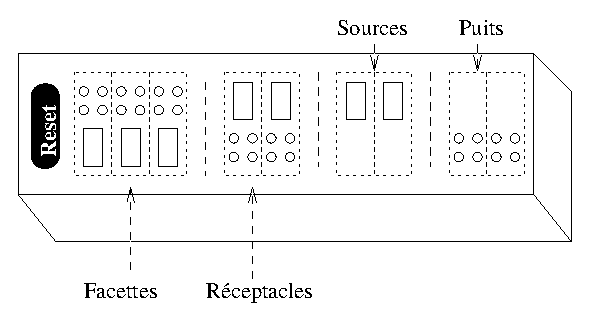
\includegraphics{figures/component-tester.eps}    
     \caption{Testeur de composant}
     \label{fig-tester-composant}
 \end{figure}

 L'\textsf{IUT} est donc  vu comme une
 bo\^{\i}te noire dont le seul comportement observable est donn\'e par
 les diff\'erents \'ecrans accessibles. Ce sc\'enario de test ne
 d\'efinit bien \'evidemment pas le comportement du testeur, c'est
 \`a dire la mani\`ere dont celui-ci agit en poussant les boutons en
 fonction des informations produites par le sc\'enario de  test. 

Le comportement du testeur est bien \'evidemment d\'etermin\'e par
la sp\'ecification que l'on souhaite v\'erifier, autrement dit par
un ensemble d'automates \textsf{FIDL} synchronis\'es. Parmi tous ces
automates nous distinguerons les cat\'egories suivantes :  
\begin{itemize}
  \item les automates dits \emph{actifs} sont moteurs dans le
  processus de test. C'est en fonction d'eux qu'est calcul\'ee la
  fonction d'\'evaluation ;
\item les automates \emph{passifs} ne jouent aucun r\^ole dans le
  processus de d\'ecision, ils peuvent \^etre amen\'e \`a
  r\'eagir  aux sollicitations de l'\textsf{IUT} ou produire des
  messages permettant au processus de test de progresser en fonctions
  des contraintes de synchronisation.
\end{itemize}

De plus, nous distinguerons les automates dits bien form\'es  dont le
comportement est une alternance d'entr\'ees et de sorties des
automates quelconques dont les entr\'ees/sorties peuvent \^etre
arbitrairement entrelac\'ees. Les premiers correspondent \`a la
sp\'ecification du comportement d'une interface et les seconds \`a
une partie du comportement d'un composant.

\subsection{Algorithme g\'en\'eral}

Pour prendre en compte l'existence de plusieurs ports de communication
et de plusieurs automates synchronis\'es repr\'esentant la
sp\'ecification, il est n\'ecessaire de modifier substantiellement l'algorithme de
base de la figure \ref{fig-algo-test-base}. Cet algorithme est
fondamentalement s\'equentiel alors qu'un composant est
potentiellement constitu\'e de flots d'ex\'ecution parall\`eles,
m\^eme si le degr\'e de parallelisme est restreint par les
synchronisations entre ports.

Le principe de fonctionnement de cet algorithme est le suivant :
\begin{itemize}
  \item parmi l'ensemble des automates synchronis\'es, un est
    distingu\'e comme \'etant l'automate actif $A$ ;
  \item comme pr\'ec\'edemment, une fonction \textsf{select} de
    s\'election de la prochaine action \`a effectuer est
    appel\'ee mais cette fois uniquement en fonction de l'automate
    actif $A$. Cette fonction retourne soit le symbole
    \textsf{terminate},
    soit le symbole \textsf{reset}, soit un ensemble ordonn\'e
    \textsf{acts} de lettres de $\Sigma_A$ ;
  \item pour chacune de ces lettres, on essaye de construire une
    s\'equence de synchronisation dans l'ensemble des automates
    $S$ : 
    \begin{itemize}
      \item si aucune s\'equence de synchronisation ne peut \^etre
        construite apr\`es \'epuisement de \textsf{acts}, alors la
        s\'equence de test courante indique une \emph{erreur dans la
          sp\'ecification} et le processus de test est arr\^et\'e,
      \item sinon, on r\'ealise les actions de
        la s\'equence $\sigma$ jusqu'\`a atteindre l'\'el\'ement de
        \textsf{acts} synchronis\'e ou jusqu'\`a ce qu'un d\'ecalage
        (conforme) soit constat\'e sur un message de sortie, et on
        recommence la proc\'edure. La figure \ref{fig-algo-execute}
        d\'etaille l'ex\'ecution de la s\'equence de synchronisation.
    \end{itemize}
\end{itemize}


\begin{figure}[htbp]
    \centering
 \begin{lstlisting}[linewidth=\textwidth,mathescape=true,numbers=left,numberstyle=\tiny,literate={:=}{{$\leftarrow$}}1 ]
 Input : $S=\{A_i = (Q_i,q_0^i,\Sigma_i,\delta_i), 1\leq i \leq n\}$
         $A \in S$  // un automate actif dans la sp\'ecification
         $I$ une implantation sous test          
 Output : failures     
 T := $\emptyset$
 Trace := $\epsilon$ 
 State := $(q_0^1,\dots, q_0^n)$ 
 Failures := $\emptyset$
 outerloop:
  while true 
    action := select(A,State,T,Trace)
    switch action
       case terminate: 
           return Failures
       case reset:
           T := T $\cup \{\mathsf{Trace}\}$
           State := $(q_0^1,\dots, q_0^n)$
           Trace := $\epsilon$
       case $acts \subset \Sigma_A$ :
            for each act $\in acts$ 
               word := $\epsilon$
               letter := $a$
               explore(State) 
               if word != $\epsilon$ then
                  execute(word)
                  continue outerloop 
               end
            end
            // problem
            return Failures
      end  
   end 
 \end{lstlisting}
 \caption{Algorithme de test de composants \textsf{FIDL}}
 \label{fig-algo-test-fidl}
 \end{figure}

Cet algorithme utilise une proc\'edure de recherche \textsf{explore} d'un mot
permettant de synchroniser plusieurs automates et se terminant par une
lettre particuli\`ere. Le principal int\'er\^et de l'agorithme est
qu'il \'evite de calculer un porduit de synchronisation global et
donc une sp\'ecification globale du composant test\'e.

\begin{figure}[htbp]
    \centering
 \begin{lstlisting}[linewidth=\textwidth,mathescape=true,numbers=left,numberstyle=\tiny,literate={:=}{{$\leftarrow$}}1 ]
function execute(word,S,I,State,Trace)
                  for $i \in \{1,\dots,\# word\}$ 
                     if word[i] $\in Out(\Sigma_S)$        
                        out := output(I) 
                        if out != $\theta$ then
                           Trace := Trace.out
                            //  unexpected output 
                            if $out \not\in \delta(State)$ then 
                               Failures := Failures $\cup$ Trace
                               T := T $\cup \{\mathsf{Trace}\}$
                               State := $q_0$
                               Trace := $\epsilon$
                            else if out $\neq$ word[i]
                               State := fire(out)
                               continue outerloop  // recommence la
                                                   // proc\'edure de d\'ecision
                             end
                        else 
                           //  a deadlock  
                           Trace := Trace.$\theta$
                           Failures := Failures $\cup$ Trace
                           T := T $\cup \{\mathsf{Trace}\}$
                           State := $q_0$
                           Trace := $\epsilon$
                        end
                     else if ! input(I,word[i]) 
                        //  refused input 
                        Trace := Trace.$\theta$
                        Failures := Failures $\cup$ Trace
                        T := T $\cup \{\mathsf{Trace}\}$
                        State := $q_0$
                        Trace := $\epsilon$
                     else
                        Trace := Trace.word[i]
                        State := fire(S,action)
                     end
                  end
                  // continue
 \end{lstlisting}
 \caption{Ex\'ecution d'une s\'equence de synchronisation}
 \label{fig-algo-execute}
 \end{figure}

Cette restriction est bien \'evidemment incorrecte dans le cas
g\'en\'eral o\`u les contraintes sont des fonctions arbitraires
puisque la r\'esolution d'un ensemble de contraintes peut d\'ependre
d'un certain nombre de \emph{tour de boucles} dans l'automate, par
exemple lorsque la contrainte d\'epend de calculs fait sur la trace.

On va donc choisir l'approche moins puissante mais dans la majorit\'e
des cas plus efficace consistant \`a s\'electionner un mot candidat
\`a l'aide de l'algorithme donn\'e puis \`a r\'esoudre les
contraintes restantes pour instancier les variables.

On notera que dans le cas d'automates \textsf{FIDL}, et de mani\`ere
plus g\'en\'eral dans le cas d'\textsf{IOLTS}, la d\'ecouverte d'un
mot permettant de synchroniser diff\'erents automates sur un objectif
commun n'est aucunement une garantie que l'action correspondant \`a
la lettre recherch\'ee soit effectivement r\'ealis\'ee dans le cas
o\`u certains des automates consid\'er\'es sont ind\'etermin\'e
en sortie pour des \'etats atteints par le mot de synchronisation. 
 
\subsubsection{Conformit\'e des ports synchrones}

La premi\`ere phase de la v\'erification de la conformit\'e d'un
composant consiste donc \`a tester celui-ci par rapport \`a la
sp\'ecification de chacun de ses ports. Dans ce cas de figure,
l'automate correspondant au port verifi\'e est consid\'er\'e comme
actif et tous les autres automates impliqu\'es dans la sp\'ecification
du composant sont passifs. 

\subsubsection{Conformit\'e du composant}

Dans une deuxi\`eme phase, la conformit\`e de l'\textsf{IUT} au
comportement sp\'ecifi\'e par le composant est v\'erifi\'ee pour
chacun des automates synchronis\'es de la sp\'ecification du
composant. Chacun alternativement est donc l'automate actif au cours
d'une session de test et tous les autres automates sont passifs. 

\section{Conclusion}

L'approche que nous proposons se distingue des travaux existant sur le
test d'\textsf{IOLTS} par l'absence de sp\'ecification globale est la
volont\'e de ne pas construire celle-ci. Cette approche se situe
ainsi \`a mi-chemin des strat\'egies de test bas\'ees sur la
d\'efinition d'un objectif de test ad-hoc par le concepteur et des
strat\'egies de test syst\'ematiques bas\'ees sur la satisfaction
d'un crit\`ere de couverture. De la premi\`ere, nous conservons la
taille relativement faible des suites de test et des testeurs en ne
testant \`a chaque \'etape qu'une partie de la
sp\'ecification. Mais l'utilisation d'une strat\'egie
d'\'evaluation des cas de test par une fontion arbitraire
d\'efinissant un certain degr\'e de couverture permet de conserver
au test unitaire de composants son caract\`ere syst\'ematique. 

Bien entendu, en l'absence de couverture compl\`ete du comportement
du composant, on ne peut tirer du r\'esultat d'une telle proc\'edure
de test que des conclusions dont la valeur d\'epend de la confiance
mise dans les crit\`eres d'\'evaluation choisis par le testeur.

%% Nous allons dans ce chapitre d\'efinir une strat\'egie
%% de s\'election des ex\'ecutions de tests applicable \`a l\'{}ensemble des
%% objectifs de test d\'efinis pr\'ec\'edemment. Cette strat\'egie
%% doit nous permettre d'atteindre deux buts contradictoires :
%% \begin{itemize}
%%   \item minimiser l'effort de test ;
%%   \item maximiser la fiabilit\'e du r\'esultat obtenu.
%% \end{itemize}
%% Pour ce faire, nous allons d\'efinir diff\'erentes mesures \`a
%% partir d\'{}une sp\'ecification sous forme d'automate \textsf{FIDL} :
%% une \emph{distance} entre les diff\'erentes ex\'ecutions possibles de
%% l'automate, et une \emph{complexit\'e} de diff\'erentes parties de
%% la sp\'ecification. Ces deux mesures seront int\'egr\'ees pour
%% construire une fonction d'\'evaluation, elle-m\^eme utilis\'ee
%% comme heuristique dans un algorithme de recherche de type
%% \textsc{Minimax}. La combinaison de ces deux mesures doit nous
%% permettre d'assurer d'une part un certain  degr\'e de
%% \emph{couverture} de la sp\'ecification, et d'autre part d'optimiser
%% l'effort de test en faisant porter celui-ci sur les parties de la
%% sp\'ecification les plus pathog\`enes. 

%% \section{Distance}
%% \label{sec:distance--limite}

%% Nous avons vu dans le chapitre \ref{chap-etatarttest} le r\^ole que
%% jouent les notions de \emph{couverture} et de \emph{crit\`ere} dans
%% le test dit structurel. Nous avons remarqu\'e par ailleurs que ces
%% notions devenaient pertinentes dans le test fonctionnel du fait de la
%% complexit\'e croissante des sp\'ecifications. \`A partir d'une certaine taille,
%% il devient infaisable d'appliquer des algorithmes exhaustifs pour
%% \'etablir la conformit\'e d'une application avec sa
%% sp\'ecification. Un certain nombre de travaux proposent des
%% crit\`eres, inspir\'es du test structurel, pour \'etablir la
%% conformit\'e avec un mod\`ele, qu'il soit sous forme d'\textsf{EFSM}
%% ou de \textsf{(IO)LTS}.

%% Nous nous basons sur ces travaux pour proposer une mesure de la
%% \emph{distance} entre mots d'un langage et donc de la
%% \emph{couverture} d'un langage par un ensemble de mots qui soit
%% effectivement calculable, intuitivement simple et pertinente et qui
%% constituera un outil efficace de s\'election des cas de tests dans un
%% algorithme de test \emph{online}. Cette distance est bas\'ee sur le
%% principe du calcul de la fonction de \emph{Parikh} que nous introduirons tout d'abord. Nous d\'efinissons
%% ensuite une mesure de la couverture entre mots et montrons que cette
%% mesure est pertinente et permet d'approcher d'aussi pr\`es que l'on
%% veut un langage --- rationnel --- quelconque. Nous terminons cette
%% section par le d\'etail des algorithmes nous permettant de manipuler
%% cette notion dans le cadre du test. 

%% \subsection{Graphes \& Matrices}

%% La matrice associ\'ee \`a un graphe $G$ dite aussi \emph{matrice
%% d'adjacence} est la matrice carr\'ee $M\in \mathbb{B}^{S \times{}S}$ telle
%% que $\forall s_i,s_j \in S$, 
%% $$
%% M_{s_i,s_j}=
%% \left\{\begin{array}{ll}
%% 1,&\mbox{~si~} \exists e \in E,\iota(e) = s_i,
%% \omega(e)=s_j \\
%% 0,&\mbox{~sinon~}.
%% \end{array}\right.
%% $$

%% La \emph{matrice d'incidence} d'un graphe $G=(S,E)$ est la matrice $I$
%% de dimension $n\times{}m$ o\`u $m=\vert E \vert$, telle que :
%% $$
%% I_{s_i,e_j} = \left\{
%%     \begin{array}{ll}
%%         -1,\mbox{~si~} \iota(e_j) = s_i \\
%%         +1, \mbox{~si~} \omega(e_j) = s_i \\
%%         0, \mbox{~sinon~}. 
%%     \end{array}\right.
%% $$

%% %% Soit $X\subset S$ un ensemble de sommets, $\omega^+(X)$ est l'ensemble
%% %% des arcs incidents ext\'erieurs  \`a $X$ 
%% %% $$
%% %% \omega^+(X) = \{a\in A\mid \iota(a)\in X, \tau(a)\not\in X\}.
%% %% $$ 
%% %% De m\^eme, $\omega^-(X)$ est l'ensemble des arcs incidents
%% %% int\'erieurs \`a $X$ :
%% %% $$
%% %% \omega^-(X) = \{a\in A\mid \iota(a)\not\in X, \tau(a)\in X\}.
%% %% $$ 
%% %% $\omega(X)= \omega^+(X) \cup \omega^-(X)$ est l'ensemble des arcs
%% %% incidents \`a $X$. 

%% %% Un \emph{cocycle} est un ensemble d'arcs incidents \`a $X$
%% %% $\omega(X)$. Un cocycle est \'el\'ementaire s'il est constitu\'e de
%% %% l'ensemble des arcs reliant entre eux deux sous-graphes connexes de
%% %% $G$. 

%% Soit $f:E\rightarrow \mathbb{Z}$ (ou dans $\mathbb{H}$ un
%% groupe quelconque) une application. Pour  chaque \'el\'ement $s$ de $S$, on
%% d\'efinit la valeur de $f$ en $s$ : 
%% $$
%% f[s] \stackrel{\mathrm{def}}{=} \sum_{(s,s')\in E} f((s,s')) -
%% \sum_{(s',s)\in E} f((s',s))
%% $$
%% L'application $f$ est un \emph{flot} si 
%% $$
%% \forall s\in S, f[s] = 0.
%% $$
%% Cette propri\'et\'e de conservation des flux entrants et sortants
%% est appel\'ee loi de \emph{Kirchoff}. 

%% Un $(s,t)$-flot pour tout couple de sommets $s$ et $t$ est une
%% application $f:E\rightarrow \mathbb{Z}$, not\'e $(f,s,t)$ telle que : 
%% $$
%% \forall q\in S, f[q] = \left\{
%%     \begin{array}{ll}
%% -1, \mbox{~si~} q=s, \\
%% +1, \mbox{~si~} q=t, \\
%% 0, \mbox{~sinon.} \\
%%     \end{array}\right.
%% $$

%% Un flot $(f,s,t)$ sera dit \emph{connect\'e} si le sous
%% graphe de $G$ induit par l'ensemble des arcs $E'=\{e\in E\mid f(e)\neq
%% 0\}$ est connexe. Un $(s,t)$-flot $(f,s,t)$ peut \^etre
%% ttransform\'e en un flot $f$ en ajoutant un arc $(t,s)$ tel que
%% $f((t,s) = 1$.

%% \subsection{Fonction \& Vecteur de Parikh}

%% Soit $\Sigma$ un alphabet fini totalement ordonn\'e de taille $k$, l'\emph{application de Parikh}\cite{parikh-cf} est un morphisme
%% $\Psi:\Sigma^* \rightarrow \mathbb{N}^k$, avec 
%% \begin{align*}
%% \forall a_i\in \Sigma, \Psi(a_i) = \left(
%%     \begin{array}{c}
%% x_1\\ x_2 \\ \vdots \\ x_k
%% \end{array}
%% \right) \mbox{~avec~} x_i=1, x_j=0
%% \mbox{~pour~} j\neq i,
%% &\mbox{~et~}&
%% \begin{array}{rl}
%% \Psi(\epsilon) &=\vec{0} \\\
%% \Psi(u.a) &= \Psi(u)+\Psi(a).\\
%% \end{array}
%% \end{align*}

%% Pour tout $u$, $\Psi(u)$ est appel\'e \emph{vecteur de
%%   Parikh}. Par extension, on notera $\Psi(L)=\{\Psi(u), u \in L\}$ l'image d'un langage
%%   $L$.  

%% \subsubsection{Ensembles lin\'eaires \& semilin\'eaires}

%% Un ensemble $L\in \mathbb{N}^p$ est lin\'eaire ssi il existe une \emph{base} 
%% $\vec{b}\in \mathbb{N}^p$ et un ensemble fini de \emph{phases} 
%% $P=\{\vec{p}_1,\dots,\vec{p}_1\} \subseteq \mathbb{N}^p$ tels que
%% $L=\{\vec{x} \mid \vec{x} = \vec{b} + \sum_{i=1}^k \lambda_i
%% \vec{p}_i, \lambda_i\in \mathbb{N}\}$. Un ensemble \emph{semilin\'eaire} est
%% une union finie d'ensembles lin\'eaires. On notera un ensemble lin\'eaire $(c,P)$ o\`u $c$ est
%% une constante --- la base --- et $P$ un ensemble \'eventuellement
%% vide de \emph{phases}, et un ensemble semilin\'eaire $\cup_{i=1}^n
%% (c_i,P_i)$. 

%% D'apr\`es le th\'eor\`eme de Parikh, pour tout langage
%% alg\'ebrique et donc pour tout langage
%% rationnel, l'ensemble des vecteurs de
%% Parikh de ce langage, c'est \`a dire l'ensemble 
%% $\Psi(L)$ est semilin\'eaire. On peut voir l'ensemble $\Psi(L)$
%% comme une repr\'esentation sous forme alg\'ebrique de l'ensemble des
%% cycles --- les phases --- possibles dans le langage $L$. Toute solution de l'un ou l'autre des
%% syst\`emes d'\'equations de l'ensemble semilin\'eaire est l'image
%% de Parikh d'un ou plusieurs mots du langage $L$. 

%% Pour obtenir l'application de Parikh pour un langage donn\'e, il est
%% donc n\'ecessaire  de construire les langages lin\'eaires d\'efinissant
%% $\Psi(L)$. 
%% Cette construction peut se faire  \`a partir de l'expression
%% rationnelle du langage\cite{litow-semilinear,lugiez-semilinear}. Si $E$ est une expression rationnelle sur un alphabet
%% totalement ordonn\'e $\Sigma$ de taille $k$ et $\Psi:\Sigma^* \rightarrow \N^k$ la
%% fonction de Parikh associ\'ee, on construit inductivement un
%% semilin\'eaire, c'est \`a dire un ensemble fini d'\'equations lin\'eaires \`a coefficients dans $\N^k$
%% permettant de calculer l'image de Parikh du langage $L(E)$ de la
%% mani\`ere suivante. Soit 
%% \begin{align*}
%%     \Psi(E) = \bigcup_{i=1}^n (c_{i},P_i) &\mbox{~et~}& \Psi(F) = \bigcup_{j=1}^m (c_{j},P_j),
%% \end{align*}
%% alors :
%% \begin{align*}
%%     \Psi(E+F) &= \Psi(E) \cup \Psi(F) \\
%%     \Psi(E^*) &= \bigcup_{i=1}^n (0,P_i\cup \{c_{i,0}\}) \\
%%     \Psi(E.F) &= \bigcup_{i=1}^n \bigcup_{j=1}^m (c_{i}+c_{j},P_i \cup P_j)\\
%%     \Psi(a) &= (\vec{a}_i,\emptyset).
%% \end{align*}
%% On remarque que cette construction est simple mais co\^uteuse puisque la
%% concat\'enation provoque une croissance exponentielle du nombre
%% d'\'equations. Elle permet toutefois d'\'eviter la construction
%% explicite de l'automate \'equivalent \`a une expression rationnelle
%% $E$ qui est aussi une op\'eration co\^uteuse.

%% \subsubsection{Image de Parikh \& Graphes}

%% \cite{seidl-icalp04} s'int\'eresse \`a la construction, \`a partir
%% d'un automate non-d\'eterministe $A=(Q,q_0,T,\Sigma,\delta)$, d'une formule
%% de l'arithm\'etique de \emph{Presburger} quantifi\'ee
%% existentiellement dont les mod\`eles sont les
%% vecteurs de Parikh du langage reconnu par l'automate. Rappelons que 
%% les ensembles
%% semilin\'eaires sont les mod\`eles des formules de l'arithm\'etique
%% de Presburger, c'est \`a dire de l'arithm\'etique sur l'ensemble
%% $\N$ utilisant uniquement l'op\'erateur $+$ et la comparaison
%% $\leq$. 

%% L'algorithme propos\'e se base sur la d\'efinition d'un \emph{flot}
%% dans le graphe sous-jacent \`a un automate ce qui permet d'obtenir le
%% r\'esultat suivant :

%% \begin{prop}[\cite{seidl-icalp04}, app. A.1]
%% \label{thr:seidl}
%% Soit $L_A$ le langage reconnu par un automate $A$ sur un alphabet
%% $\Sigma$ totalement ordonn\'e de taille $k$. Un vecteur $\vec{u} \in
%% \N^k$  est dans l'image de Parikh de $L_A$, ssi
%% il existe un \emph{$(q_0,t)$-flot connect\'e} $(f,q_0,t)$, pour
%% $q_0$ l'\'etat initial de $A$ et $t\in T$ un \'etat terminal, et
%% $f:\delta\rightarrow \N$ une application tels que :
%% $$
%% \forall a\in \Sigma, \vec{u}[a] = \sum_{q \in \delta(p,a)} f(p,a,q).
%% $$ 
%% \end{prop} 

%% \subsection{Applications aux automates}

%% Nous nous basons sur les d\'efinitions et r\'esultats
%% pr\'ec\'edents concernent les vecteurs de Parikh pour d\'efinir une
%% notion diff\'erente mais connexe : l'ensemble des vecteurs
%% repr\'esentant les diff\'erentes \emph{transitions} de l'automate
%% qu'il est possible de franchir en reconnaissant un mot. Nous
%% appelerons les \'el\'ements de cet ensemble des \emph{P-vecteurs} et
%% l'ensemble lui-m\^eme un \emph{P-ensemble}.  On
%% constatera que la construction d'un P-ensemble pour un langage est similaire \`a la
%% construction de l'ensemble des images de Parikh d'un langage, \`a un
%% re\'etiquetage pr\`es des lettres du langage pour distinguer les
%% diff\'erentes occurences de lettres sur diff\'erentes transitions. 

%% L'objectif de cette section est de caract\'eriser : 
%% \begin{itemize}
%%   \item l'ensemble des P-vecteurs qui sont l'image des mots
%%     reconnus par un automate ;
%%   \item l'ensemble des mots qui ont pour P-vecteur un certain
%%   vecteur $\vec{v}$.
%% \end{itemize}

%% Soit un automate fini
%% d\'eterministe $A=(Q,q_0,T,\Sigma,\delta)$ et son langage
%% $L_A$. Soit $G=(Q,E)$ le
%% graphe de l'automate $A$, \`a chaque arc $(q,q')\in E$ est
%% associ\'e un indice entre $1$ et $m = \mid E\mid$ de sorte que $E$ soit
%% totalement ordonn\'e. Nous utiliserons indiff\'eremment des
%% \'el\'ements de $E$ ou des entiers en tant qu'indices. 

%% Nous d\'efinissons $\psi$, la fonction permettant de construire le
%% P-ensemble pour le langage d'un automate $A$. $\psi:E \rightarrow
%% \N^{m+1}$, est d\'efinie comme :
%% $$
%% \psi(e_i) = \left(
%%     \begin{array}{c}
%% 0 \\x_1\\ x_2 \\ \vdots \\ x_{m}
%% \end{array}
%% \right) \mbox{~avec~} x_i=1 \mbox{~et~} x_j=0
%% \mbox{~pour~} j\neq i. 
%% $$
%% On notera $\mathbf{1}$ le vecteur $(1,0,\dots,0) \in  \N^{m+1}$ et
%% $\mathbf{0}$ le vecteur $(0,0,\dots,0)$. Le lecteur attentif aura
%% remarqu\'e que le vecteur est de taille $m+1$. L'utilit\'e de cette
%% dimension suppl\'ementaire appara\^{\i}tra plus clairement dans la
%% section consacr\'ee \`a la distance.

%% L'application $\psi$ est \'etendue aux  mots $u \in Pref(L_A)$,
%% repr\'esent\'es par un chemin $e_1e_2 \dots e_k$ de longueur $k$ dans l'automate
%% $\cal A$ de la mani\`ere suivante :
%% $$
%% \psi(e_1e_2\dots e_k) = \sum_{j=1}^k\psi(e_j) + \left\{
%%     \begin{array}{ll}
%% \mathbf{1}, \mbox{~si~} \omega(e_k) \in T, \\
%% \mathbf{0}, \mbox{~sinon~}. \\
%%     \end{array}\right.
%% $$
%% Tout mot $u$ de $L_A$ est donc repr\'esent\'e comme un vecteur de $m+1$
%% \'el\'ements \`a coefficients entiers repr\'esentant le nombre
%% d'occurences de chaque transition franchie pour reconna\^{\i}tre $u$
%% dans $A$.  Bien \'evidemment, l'application $\psi$ n'est pas
%% g\'en\'eralement injective : \`a plusieurs mots peuvent 
%% correspondre un m\^eme vecteur. 

%% \subsubsection{Repr\'esentation matricielle de $\psi(L_A)$}

%% On va caract\'eriser $\psi(L_A)$, le P-ensemble associ\'e \`a $A$ pour faire
%% correspondre \`a chaque vecteur $\vec{v}=(1,v_1,\dots,v_m)\in \N^{m+1}$ l'ensemble des
%% mots $v$ de $L_A$ tels que $\psi(v) = \vec{v}$. Ce vecteur correspond
%% \`a un mot $v$ si et seulement si il existe un chemin $\sigma$ dans
%% l'automate $A$ de $q_0$ vers $q$ avec $\vert \sigma \vert =
%% \sum_{i=1}^m v_i - 1$. Le th\'eor\`eme \ref{thr:seidl}
%% caract\'erise $\Psi(L_A)$  par les
%% propri\'et\'es d'un flot entre $q_0$ et un \'etat terminal de
%% $A$. Nous nous basons sur cette d\'efinition pour d\'ecrire
%% $\psi(L_A)$ comme l'ensemble des solutions d'un syst\`eme lin\'eaire
%% d'\'equations poss\'edant une certaine structure. 

%% On va se servir de la
%% \emph{matrice d'incidence} du graphe de l'automate $\cal A$ \'etendue
%% \`a $m+1$. Cette extension est not\'ee $\mathfrak{M}$ et d\'efinie
%% comme :
%% $$
%% \mathfrak{M} = 
%% \left(\begin{array}{cc}
%%         1 & 0 \\
%%         0 & \fbox{I} 
%%     \end{array}\right).
%% $$ 

%% Un vecteur $\vec{v} \in \N^{m+1}$ est un P-vecteur s'il est
%% solution d'une \'equation : 
%% \begin{equation}
%% \mathfrak{M}. \vec{X}  = S_t,\label{eq:sys-parikh}
%% \end{equation}
%% o\`u $X$ est un vecteur colonne de $m+1$ \emph{variables} distinctes
%% et $S^t$ est une famille de vecteurs indic\'ee par les \'el\'ements
%% de $T$, l'ensemble des \'etats terminaux de l'automate $A$ 
%%  de taille $\N^{1+Q}$  tel que :
%% \begin{align*}
%% S_1^t = 1 \quad&\mbox{et}&\quad   S_{q_i} = \left\{
%%     \begin{array}{ll}
%% -1,&\mbox{~si~} q_i=q_0 \\
%% +1,&\mbox{~si~} q_i=t\\
%% 0,&\mbox{~sinon~}.
%%     \end{array}\right.
%% \end{align*}

%% Autrement dit, on a un syst\`eme lin\'eaire de $n$ \'equations et
%%  $m$ variables \`a r\'esoudre pour trouver le ou
%% les mots  $v$ correspondant au vecteur $\vec{v}$. 
%% Ce syst\`eme exprime le fait que :
%% \begin{itemize}
%%   \item tout vecteur est un \emph{flot} et par cons\'equent la somme
%%     des poids des arcs entrant et sortant doit \^etre 0 sauf pour
%%     l'\'etat de d\'epart et l'\'etat d'arriv\'ee du flot. Cette
%%     condition s'exprime facilement comme un syst\`eme d'\'equations
%%     lin\'eaires induit par la matrice d'incidence $I$ ;
%%   \item pour l'\'etat de d\'epart et celui d'arriv\'ee, la valeur total des poids
%%     associ\'es aux arcs entrants  et sortants est respectivement de
%%     $-1$ et $1$. 
%% \end{itemize}
%% Comme il peut exister plusieurs \'etats terminaux, plusieurs
%% solutions sont possibles et il est donc n\'ecessaire de distinguer
%% les diff\'erentes possibilit\'es d'attieindre un \'etat terminal. 

%% Dans le cas o\`u l'automate $A$ a un seul \'etat terminal $t$, alors
%% la matrice $\mathfrak{M}$ peut \^etre red\'efinie comme 
%% $$
%% \mathfrak{M} = 
%% \left(\begin{array}{cc}
%%         1 & 0 \\
%%  \fbox{$S_t$} & \fbox{$I$}  \\
%%     \end{array}\right)
%% $$ 
%% et l'\'equation \eqref{eq:sys-parikh} se r\'e\'ecrit plus
%% simplement comme 
%% \begin{equation}
%%     \label{eq:sys-parikh-normal}
%% \mathfrak{M}. \vec{X} = \mathbf{0}.
%% \end{equation}

%% Cette condition est n\'ecessaire mais n'est pas suffisante car elle
%% n'exprime pas l'exigence de connexit\'e entre tous les \'etats
%% participant du flot. On peut exprimer le fait qu'un P-vecteur
%% repr\'esente un chemin connexe en le comparant aux plus petits
%% chemins permettant d'atteindre chacune des transitions parcourues par
%% le P-vecteur. 

%% Pour tout arc $e_i=(q',q)$, soit
%% $c(e_i)$ l'ensemble des P-vecteurs des $(q_0,q)$-chemins $\mu{}$ tels que
%%  $\vert \mu{}\vert = k$ et $E(\mu{})[k-1]=e_i$:
%% $$
%% c(e_i) = \{\psi(u) \mid u=va, q_0 \xrightarrow{v} q'
%% \xrightarrow[e_i]{a}, \mbox{~et $v$ est minimal~}\}.
%% $$
%% Alors, tout P-vecteur $\vec{v}=(1,v_1,\dots,v_m)$ solution de l'\'equation
%% \eqref{eq:sys-parikh} doit de plus v\'erifier la condition suivante :
%% \begin{equation}
%%     \label{eq:parikh-connect}
%%     \forall v_i \neq 0, \exists \vec{c}\in c_i, \vec{c}\leq \vec{v},
%% \end{equation}
%% o\`u $\vec{w}\leq \vec{v}$ si et seulement si $\forall i,1\leq i\leq m, w_i\leq v_i$.

%% \paragraph{Exemple}

%% Par exemple, soit l'automate pr\'esent\'e dans la figure
%% \ref{fig-sample-dfa-distance} o\`u les transitions sont indic\'ees
%% de la mani\`ere suivante :
%% $$
%% \begin{array}{rcl}
%% (2 , b , 0)&\mapsto &1\\
%%  (3 , b , 0)&\mapsto &2\\
%% (1 , a , 3)&\mapsto &3\\
%%  (3 , c , 0)&\mapsto &4\\
%%  (0 , a , 2)&\mapsto &5,
%% \end{array}
%% $$
%% le vecteur associ\'e au mot $abab$ est $(1,1,1,1,0,1)$, celui
%% associ\'e au mot $acabab$ est $(1,2,0,1,1,2)$. Le vecteur associ\'e
%% \`a $\epsilon$ est d\'efini comme $(1,0,0,0,0,0)$.

%% La matrice $\mathfrak{M}$ est 
%% $$
%% \left(\begin{array}{cccccc}
%% 1 & 0 &  0 &  0 & 0  & 0  \\
%% 0 & 1 &  1 &  0 & 1  & -1 \\
%% 0 & 0 &  0 & -1 & 0  & 0  \\
%% 0 & -1 & 0 &  0 & 0  & 1  \\
%% 0 & 0 & -1 &  1 & -1 & 0  \\
%% \end{array}\right), 
%% $$
%% et par cons\'equent l'ensemble des vecteurs de Parikh est donn\'e
%% par les solutions au syst\`eme d'\'equations suivants :
%% $$
%% \left\{\begin{array}{ccccccr}
%% x_1 &+ x_2 &&+ x_4 &- x_5  &=& 1 \\
%% &&- x_3 && &=& -1 \\
%% -x_1 &&&+ x_4 &&=& 0 \\
%% &-x_2 &+ x_3 &-x_4 &&=& 0 \\
%% \end{array}\right..
%% $$

%% \begin{figure}
%%     \centering
%% 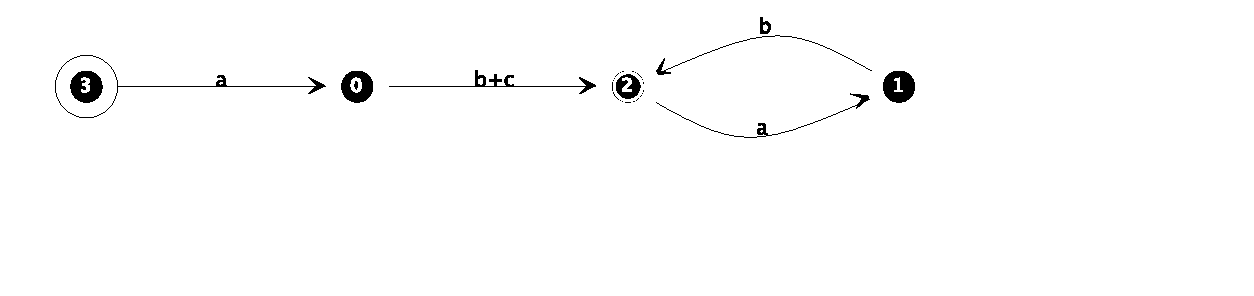
\epsfig{width=.5\textwidth,file=figures/fig-sample-dfa-distance.eps}    
%%     \caption{Automate d\'eterministe minimal pour le langage $a(b+c)(ab)^*$}
%%     \label{fig-sample-dfa-distance}
%% \end{figure}

%% \subsubsection{Calcul de $\psi^{-1}(\vec{v})$}

%% \'Etant donn\'e un vecteur de Parikh $v$ appartenant \`a l'image de
%% $L_A$, on souhaite pouvoir reconstituer le ou les mots dont $v$ est
%% l'image. Ce probl\`eme a deux formes distinctes :
%% \begin{enumerate}
%%   \item reconstuire un mot $u$ appartenant \`a $\psi^{-1}(v)$ ;
%%   \item reconstruire $\psi^{-1}(v)$.
%% \end{enumerate}

%% Le premier probl\`eme est  simple : on parcours l'automate en mettant \`a jour le vecteur en fonction des
%% transitions franchies jusqu'\`a atteindre le vecteur $\mathbf{1}$ qui
%% doit correspondre \`a l'atteinte d'un \'etat terminal. L'algorithme
%% est pr\'esent\'e dans la figure \ref{fig-algo-inverseimage} : il
%% retourne le mot construit s'il existe, c'est \`a dire si $v\in
%% \psi(L_A)$ et $\epsilon$ sinon. 

%% \begin{figure}[htbp]
%%     \centering
%%     \begin{lstlisting}[mathescape=true,literate={:=}{{$\leftarrow$}}1 ]
%% Input: $A=(Q,q_0,T,\Sigma,\delta)$ un automate 
%%        $v\in \N^{\vert \delta\vert+1}$ un vecteur  de Parikh
%% Output: un mot $u \in L_A$, si $v\in \psi(L_A)$

%% $q$ := $q_0$
%% $u$ := $\epsilon$
%% $C$ := base de cycle de $A$

%% while $v \neq \mathbf{1}$
%%    out := out(v,q)
%%    if $\vert out \vert$ > 1 then
%%        c := $\{ e \mid (n,e) \in out,e\in C\}$
%%        // verifie la correction de v
%%        c' := $\{ e \mid (n,e) \in out,e\not\in C\}$
%%        if $\vert c' \vert > 1$ then
%%           return $\epsilon$
%%        end
%%        // choisit un cycle s'il y en a un
%%        if $\vert c \vert > 0$ then 
%%           t := $e=(q,a,q') \in c$
%%        else 
%%           t := $e=(q,a,q') \in c'$
%%        end
%%        // franchit la transition
%%        u := $u.a$
%%        q := $q'$
%%        v := $v - \psi(e)$
%%    else
%%       return $\epsilon$
%%    end
%% end
%% return $u$

%% // fonction auxiliaire
%% out(v, q) $\stackrel{}{=}[\mathrm{def}] \{ (v_i,e_i) \mid v_i>0, e_i =
%% (q,q') \in E\}$

%%  \end{lstlisting}    
%%      \caption{Calcul d'un mot de $\psi^{-1}(v)$}
%%      \label{fig-algo-inverseimage}
%%  \end{figure}

%% Le second probl\`eme est  plus complexe et plus int\'eressant car il n\'ecessite de
%% calculer une op\'eration de cl\^oture commutative pour tous les
%% cycles apparaissant dans le vecteur $v$ entre deux cocycles. Dans
%% l'imm\'ediat, nous ne nous attarderons pas sur ce calcul qui
%% n\'ecessiterait des d\'eveloppements importants.

%% %% Cette repr\'esentation pr\'esente l'inconv\'enient d'\^etre assez
%% %% \og gourmande\fg alors m\^eme que certains \'el\'ements du vecteurs
%% %% sont li\'es les uns aux autres. On la raffine donc en utilisant comme
%% %% \'el\'ements du vecteurs les \emph{bases de cycle} du graphe
%% %% sous-jacent \`a l'automate $A$. Les bases de cycle d'un graphe
%% %% dirig\'e sont les chemins du graphe tels que tout autre chemin peut
%% %% s'exprimer comme une combinaison lin\'eaire d'\'el\'ements de la
%% %% base. Plus formellement :

%% %% \begin{definition}[Base de cycle d'un graphe $G$]
%% %% Pour tout graphe dirig\'e $G=(S,E)$, une base de cycle est un
%% %% ensemble $B=\{b_1,b_2, \dots,b_n\}$ de \emph{chemins \'elementaires}
%% %% ind\'ependants de $G$ tel que pour
%% %% tout chemin $p$ de $A^*$ n'appartenant pas \`a $B$,
%% %% $$
%% %% p = \sum_{i=1}^{\mid B \mid} k_i b_i, \quad k_i \in \mathbb{Q}.
%% %% $$
%% %% \end{definition} 

%% \subsection{Distance}

%% \`A partir des vecteurs repr\'esentant chaque mot dans $\N^{m+1}$, on peut
%% d\'efinir une \emph{norme} et une \emph{distance}. On d\'efinit
%% l'application $\phi:L_A \rightarrow \mathbb{Q}^{m+1}$ associant \`a
%% tout mot du langage $L_A$ un vecteur \`a coefficients dans
%% $\mathbb{Q}$, l'ensemble des nombres rationnels, de norme 1 :
%% $$
%% \phi(u) = \frac{\psi(u)}{\vert\psi(u)\vert}, \forall u\in L_A,
%% $$
%% avec 
%% $$
%% \vert\psi(u)\vert =  1+\sum_{i=1}^m x_i.
%% $$
%% On remarquera que la norme utilis\'ee est la norme dite \emph{L-1} et non la
%% norme euclidienne traditionnelle. Ce choix est justifi\'e par le fait
%% que $\psi(u)$ est une repr\'esentation de mots pour lesquels la norme
%% naturelle est la longueur. La distance induite par cette norme entre
%% deux P-vecteurs $\psi(u)$ et $\psi(v)$ est appel\'ee \emph{distance de Manhattan}.

%% Chaque $\phi(u)$ image d'un mot $u$ est donc un point sur la surface
%% d'une portion de sph\`ere
%% dans un espace \`a $m+1$ dimensions  muni d'une distance L-1 :
%% $$
%% \mathbf{d}(\vec{u},\vec{v}) = \vert\vec{u} - \vec{v}\vert_1.
%% $$

%% \begin{definition}[P-distance sur un langage reconnaissable $L$]
%%     Soit $L$ un langage reconnaissable par un automate $A$. La
%%     P-distance  entre deux mots $u$ et $v$ de $Pref(L)$, not\'ee
%%     $\mathbf{s}(u,v)$, est d\'efinie comme :
%%     $$
%%     \mathbf{s}(u,v) = \mathbf{d}(\phi{u},\phi{v}).
%%     $$
%% \end{definition}

%% De mani\`ere \'evidente, la distance $\mathbf{s}(u,v)$ sur un langage reconnaissable $L$ est une
%% m\'etrique puisque $\mathbf{d}$ est une m\'etrique sur
%% $\mathbb{Q}^{m+1}$. 
%% Intuitivement, $\mathbf{s}(u,v)$ repr\'esente un degr\'e de similitude entre
%% deux mots reconnus par $\cal A$. C'est aussi dans le cadre du test une mesure de la validit\'e d'une
%% \emph{hypoth\`ese  de r\'egularit\'e}.

%% \begin{figure}[htbp]
%%     \centering
%%  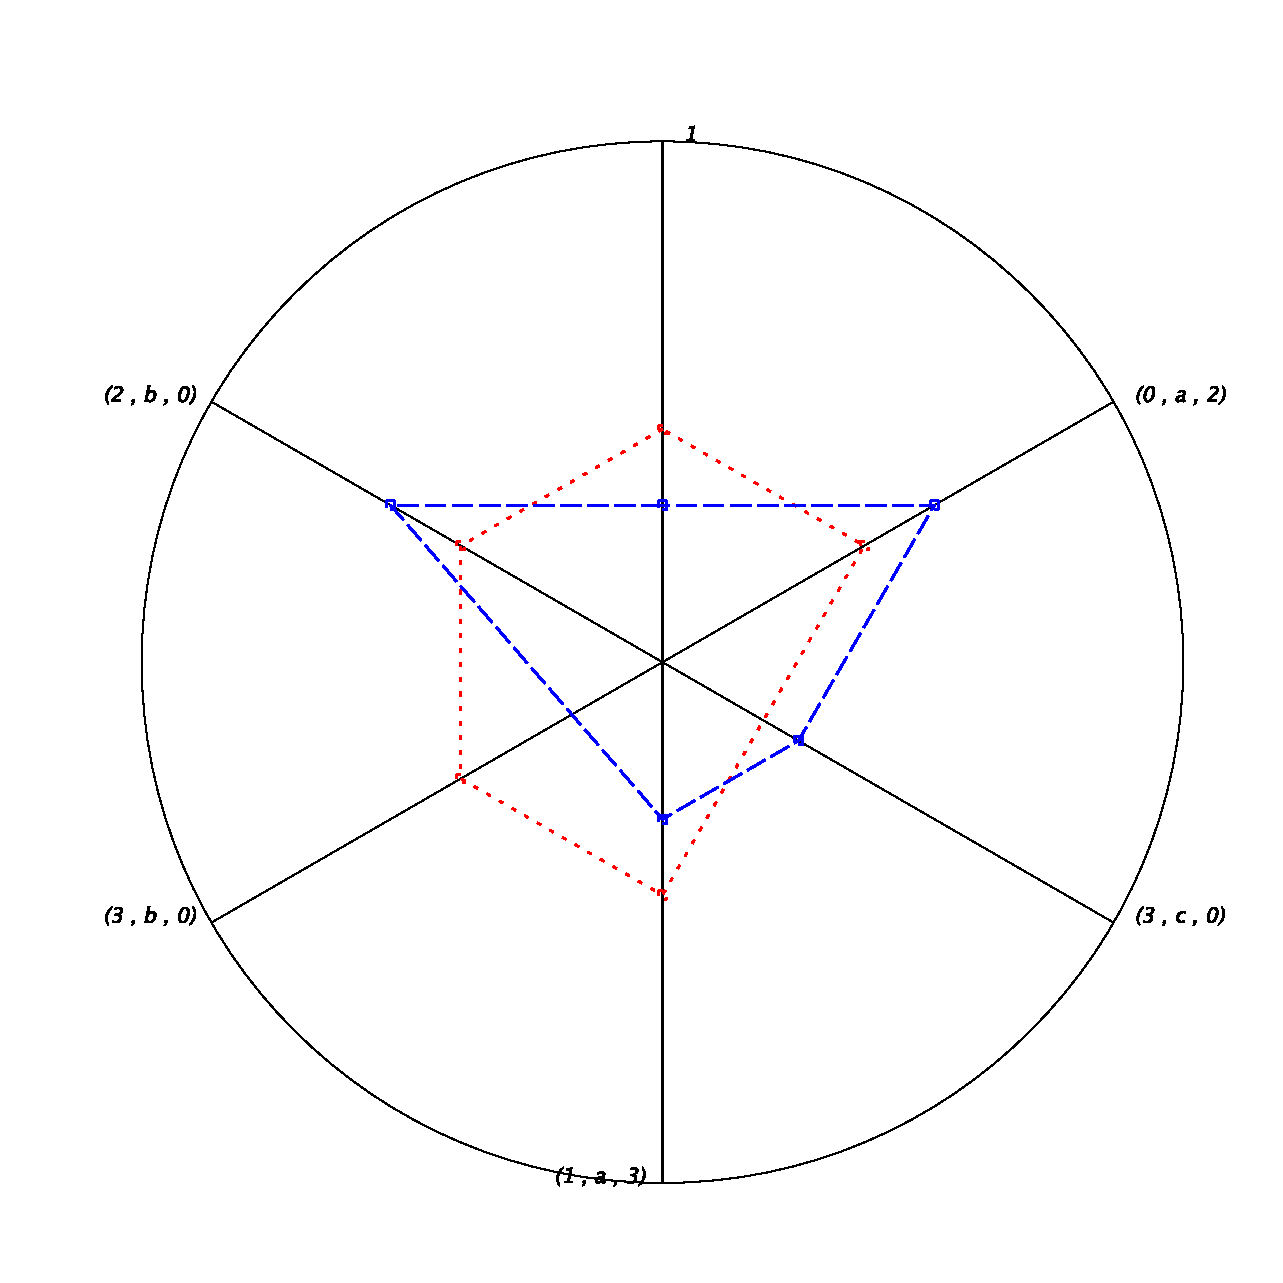
\epsfig{width=.50\textwidth,file=figures/fig-radial.eps}   
%%     \caption{Diagramme radial - Exemple}
%%     \label{fig-radial}
%% \end{figure}

%% La figure \ref{fig-radial}  est une repr\'esentation de l'espace
%% des mots pour un automate $\cal A$ sous la forme d'un diagramme
%% radial. On divise un cercle de rayon $1$ par $m+1$ rayons et
%% chaque coordonn\'ee  est repr\'esent\'ee sur le rayon
%% correspondant. Cette
%% repr\'esentation est une \og projection \fg naturelle de l'espace
%% parcouru par les vecteurs $\vec{u}$ normalis\'es plus maniable qu'une
%% projection en 2 ou 3 dimensions. Elle est rendu possible par le fait
%% que chaque coordonn\'ee est comprise entre 0 et 1. La figure
%% \ref{fig-radial} repr\'esente les diff\'erentes coordonn\'ees
%% pour le langage $a(b+c)(ab)^*$ : le trac\'e en pointill\'e
%% repr\'esente les coordonn\'ees du mot $(ab)^2$ et le
%% trac\'e en tirets le mot $ac(ab)^2$. 

%% \subsubsection{Ensemble des distances}

%% Nous supposons sans perte de g\'en\'eralit\'e que l'automate
%% $\cal A$ poss\`ede un seul \'etat terminal. L'ensemble des
%% P-vecteurs  de $L_A$, $\psi(u)$, est l'ensemble des solutions
%% dans $\N^{m+1}$ du syst\`eme d'\'equation d\'etermin\'e par la
%% matrice d'incidence de $\cal A$ :
%% $$
%% \begin{array}{cccc}
%% \left(\begin{array}{cc}
%%         1 & 0 \\
%%         S' & I 
%%     \end{array}\right)& X &=& \left(\begin{array}{cc}
%%         1  \\
%%         0 \\
%%         \vdots \\
%%         0
%%     \end{array}\right)
%% \end{array}
%% $$ 
%% o\`u $S$ est un vecteur de taille $n$ tel que $S_i=1$ si $i=q_0$ et
%% $S_i=-1$ si $i\in T$. 

%% L'ensemble $\phi(L_A)$ des
%% vecteurs  repr\'esentant les mots $u \in L_A$ est inclus dans
%% $[0,1]^{m+1}$ et il est d\'etermin\'e par 
%% l'ensemble des solutions dans $[0,1]^{m+1}$ du syst\`eme
%% d'\'equation suivant \`a coefficients dans $\mathbb{Q}$ :
%% $$
%% \begin{array}{cccc}
%% \left(\begin{array}{cc}
%%         1 & 
%%         \begin{array}{ccc}
%% 1 & \dots & 1
%% \end{array}
%% \\
%%         S' & I 
%%     \end{array}\right)& X &=& \left(\begin{array}{cc}
%%         1  \\
%%         0 \\
%%         \vdots \\
%%         0
%%     \end{array}\right).
%% \end{array}
%% $$ 

%% \subsection{$\eta$-couverture}

%% Une propri\'et\'e int\'eressante de la transposition des vecteurs
%% de $\N^{m+1}$ dans $[0,1]^{m+1}$ est de permettre de passer d'un
%% espace discret \`a un espace continu et donc de d\'efinir une
%% notion de limite pour  $\phi(u)$. Une fonction $f(x)$ poss\`ede une
%% limite $c$ en $a$ si pour tout $\epsilon > 0$, il existe $\delta > 0$ tel
%% que $\vert f(x) - c\vert < \epsilon$  quand $ 0< \vert x - a\vert <
%% \delta$. 

%% Les bornes de $\psi(u)$ forment les facettes d'un polytope convexe ouvert
%% repr\'esentant l'ensemble des  solutions de l'\'equation de $\psi(u)$. Ces sommets peuvent \^etre
%% calcul\'es par des m\'ethodes existantes de traitement des
%% polyh\`edres (voir par exemple \textsf{polylib} ou \textsf{qhull}\cite{barber96quickhull}), y compris en
%% utilisant des automates pour repr\'esenter l'ensemble des vecteurs
%% correspondant\cite{latour-auto-polyhedre}. Les bornes de $\phi(u)$
%% sont situ\'ees sur la sph\'ere en $m+1$ dimensions et sont les
%% images de l'ensemble des solutions de $\psi(u)$ par la fonction
%% $f(x)/\vert x\vert_1$. 

%% %% La partie droite de la figure \ref{fig-distance-lim} est une illustration des
%% %% propri\'et\'es de $\mathbf{s}(u,v)$ dans le cas simple de deux
%% %% dimensions. Ici, le mot $u$
%% %% est repr\'esent\'e par le vecteur $(2,1)$ et le mot $v$ par le
%% %% vecteur $(2,4)$ et l'on a donc $u=xy$ et $v=xy^4$. Dans ce cas, si on
%% %% pose $\theta = 2+i$ et $\theta'=2+4i$, on a 
%% %% $$
%% %% \vec{v} - \vec{u} = (\cos \theta' - cos\theta, \sin \theta' - \sin\theta)
%% %% $$
%% %% d'o\`u 
%% %% \begin{align}
%% %%     \mathbf{s}(u,v)^2 &= (\cos\theta' - cos\theta)^2 + (\sin
%% %%     \theta' - \sin\theta)^2 \\
%% %%     & =  \cos\theta'^{2} - 2\cos\theta'\cos\theta + \cos\theta^2 + \sin\theta'^{2} - 2\sin\theta'\sin\theta + \sin\theta^2\\
%% %%     & =  2(1 - \cos\theta'\cos\theta  - \sin\theta'\sin\theta) \label{eq:dist-mot}\\
%% %%     & =  2(1  - \cos(\theta' - \theta)) \\
%% %%     \mathbf{s}(u,v) & = \sqrt{2(1 - \cos(\theta' -
%% %%     \theta))}.
%% %% \end{align}
%% %% Si l'on consid\`ere $u=xy$ et $v=xy^k$ et en utilisant \ref{eq:dist-mot}, on a :
%% %% \begin{align}
%% %%     \lim_{k\rightarrow+\infty} \cos\theta' &= 0 \\
%% %%     \lim_{k\rightarrow+\infty} \sin\theta' &= 1 \\
%% %%     \lim_{k\rightarrow\infty} \mathbf{s}(u,v) &= 
%% %%     \sqrt{2(1-\sin\theta)}.\label{eq:lim-dist-mot}
%% %% \end{align}

%% %% \begin{figure}[htbp]
%% %% \epsfig{width=.30\textwidth,clip=,file=figures/fig-proof-triangle.eps}\hfill 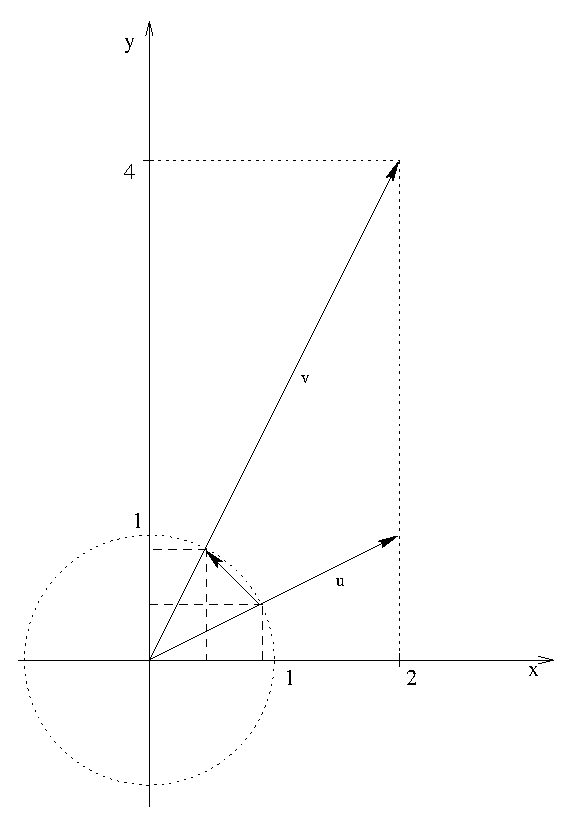
\epsfig{height=7.5cm,clip=,file=figures/fig-distance-lim.eps}
%% %%      \caption{Visualisation g\'eom\'etrique de $\mathbf{s}(u,v)$}
%% %%      \label{fig-distance-lim}
%% %% \end{figure}

%% On peut donc d\'ecrire la mani\`ere dont un
%% sous-ensemble fini du langage reconnu par $A$ \emph{couvre} le
%% langage $L$. 

%% \begin{definition}[$\eta$-couverture]
%%     Soit $T\subseteq L$ un sous ensemble des mots de $L$, $T$ est une
%%     $\eta$-couverture de $S$ si et seulement si,
%%     $$
%%     \forall u \in L, \exists t \in T, \mathbf{s}(u,t) \leq \eta.
%%     $$
%%     Clairement, $\emptyset$ est une 1-couverture de $L$ et $L$
%%     est une 0-couverture de lui-m\^eme.
%% \end{definition}

%% \begin{prop}[$\eta$-couverture]
%% Pour tout langage  $L$ reconnu par un automate $A$, pour tout
%% $\eta\in [0,1]$, il existe un langage fini $T\subseteq L$ tel
%% que $T$ est une $\eta$-couverture de $L$ : 
%% $$
%% \forall u \in L, \exists t \in T, \mathbf{s}(u,t) \leq \eta.
%% $$
%% \end{prop}

%% \begin{proof}
%% Soit $\eta$ une valeur de couverture quelconque, nous
%% construisons un ensemble fini $T$ de --- pr\'efixes de --- mots de
%% $L_A$ tel que $T$ en soit une $\eta$-couverture. 

%% Pour tout chemin \'el\'ementaire ind\'ependant $\sigma$ partant de $q_0$, l'\'etat initial
%% de $A$, on ajoute  dans $T$ le mot  $u$  construit en concat\'enant les
%% \'etiquettes des transitions composant le chemin
%% $\sigma$. Clairement, $T$ est alors une $0$-couverture de l'ensemble
%% des pr\'efixes  de mots $L_A$ ne contenant aucun facteur
%% it\'erant et c'est donc \emph{a fortiori} une $\eta$-couverture. 

%% D'apr\`es le \emph{lemme de l'\'etoile} (\cite{sakarovitch}, p.78),
%% tout mot ou facteur de mot \og suffisamment long\fg de $L_A$ contient un facteur
%% it\'erant. Soit $uv^*w$ une partie du langage de $L_A$
%% contenant un facteur it\'erant, alors d'apr\`es
%% \eqref{eq:lim-dist-mot}, on peut construire un mot
%% $y=uv^kw$ tel que pour tout $x=uv^jw \in uv^*w$, 
%% $$
%% \mathbf{s}(x,y) \leq \eta,
%% $$
%% et $T$ est donc une $\eta$-couverture de $uv^*w$. Comme
%% $L_A$ contient un nombre fini de facteurs it\'erants, $T$ est
%% fini et est donc une $\eta$-couverture de $L_A$.\hfill\qed
%% \end{proof}

%% Bien s\^ur, cette mesure de couverture est donn\'ee \emph{modulo} la
%% commutativit\'e des chemins permettant de construire des mots du
%% langage de $L_A$. Par exemple, pour le langage $(a(bc+ef)a)^*$,
%% les mots $abcaaefa$ et $aefaabca$ on m\^eme 
%% vecteur $(1,2,1,1,1,1,2)$ et sont donc \`a une distance de
%% 0. Cette commutativit\'e des chemins est induite par
%% l'ind\'ependance de certaines s\'equences de lettres, autrement dit
%% par les entrelacements d'ex\'ecution possible entre diff\'erents
%% mots. Si l'on souhaite obtenir une couverture plus fine, on peut
%% obtenir la cl\^oture commutative d'un ensemble $T$. 

%% \`A partir de cette mesure, deux questions int\'eressantes se posent :
%% \begin{enumerate}
%%   \item \'etant donn\'es un langage $L$ et un ensemble $T$, quelle est
%%     l'$\eta$-couverture de $T$ sur $L$ ? 
%%   \item \'etant donn\'es un langage reconnaissable $L$ et une
%%     couverture, $\eta$, comment g\'en\'erer un ensemble $T$ qui soit
%%     une $\eta$-couverture de $L$ ? 
%% \end{enumerate}

%% \subsubsection{Calcul de l'$\eta$-couverture de $T$}

%% L'ensemble $T\subseteq L$
%% est un ensemble fini de mots dans un langage reconnaissable donn\'e
%% repr\'esent\'e canoniquement par un automate d\'eterministe minimal
%% $\cal A$. Soit $m$ le nombre de transitions de $\cal A$, chaque mot de
%% $T$ et de $L$ est repr\'esent\'e par un vecteur de taille $m+1$ et
%% de norme 1. Par d\'efinition, la mesure de $\eta$ pour $T$ est
%% donn\'ee par la plus grande distance existant entre un mot de $T$ et
%% un mot de $L$. 

%% G\'eom\'etriquement, cette propri\'et\'e correspond \`a la
%% construction d'un \emph{diagramme de Vorono\"{\i}} \`a partir des
%% vecteurs $\phi(T)$. Pour un ensemble de
%% points $S$ dans  $\mathbb{R}^{n}$, un \emph{diagramme de
%% Vorono\"{\i}}\cite{aurenhammer-voronoi-survey} $V(S)$ est une partition de l'espace en poly\`edres
%% convexes ou \emph{r\'egions} $\mathsf{reg}(s),s\in S$ tels que que pour tout point $p\in
%% \mathsf{reg}(s)$ et pour 
%% toute r\'egion $\mathsf{reg}(s'), s\neq s'$, $d(s,p)\leq d(s',p)$. Le
%% diagramme  de Vorono\"{\i} pour $\phi(T)$ \'etant donn\'e,
%% l'$\eta$-couverture de $T$ est donn\'ee par la plus grande des
%% distances entre $t\in T$ et chacun des sommets de $\mathsf{reg}(t)$ :
%% $$
%% \eta(T) = \mathsf{max}\{ \mathbf{d}(t,p),\forall t\in T, p\in \mathsf{reg}(t)\}.
%% $$

%% L'algorithme \textsf{Quickhull}\cite{barber96quickhull} est un
%% algorithme classique et efficace de calcul d'enveloppe convexe d'un ensemble de
%% points en $n$ dimensions. Pour une dimension $d>3$ et un nombre de
%% points d'entr\'ee $n$, sa complexit\'e
%% est estim\'ee \`a $O(n^{d/2}/\lfloor d/2\rfloor!)$. Cet algorithme
%% part de la construction d'un \emph{simplex} de dimension $n$, c'est
%% \`a dire un volume r\'egulier d\'efini par $n+1$ points puis
%% il reconstruit des facettes en ajoutant un \`a un les points de
%% l'ensemble d'entr\'ee et en trouvant la facette la plus proche du
%% point ajout\'e pour la diviser. 

%% \subsubsection{Calcul de $T$ en fonction de l'$\eta$-couverture}

%% Le calcul de $T$ en fonction de $\eta$ est le dual du probl\`eme
%% pr\'ec\'edent. Si l'on reprend la d\'efinition d'$\eta(T)$
%% donn\'ee ci-dessus, on constate que cette d\'efinition d\'epend de
%% la construction d'un ensemble de r\'egions dont la plus grande
%% distance est inf\'erieure ou \'egale \`a $\eta$. Pour construire
%% $T$, on va donc tout d'abord construire un 
%% polytope convexe r\'egulier dont toutes les r\'egions ont m\^eme
%% diam\`etre, en l'occurrence $\eta$, par subdivision du simplex de base correspondant
%% aux limites pour le langage $L$ dans chacune des dimensions. 

%% On obtient ainsi les coordonn\'ees d'un
%% ensemble de vecteurs, le centre de chaque facette du polytope,
%% repr\'esentant les candidats pour $T$. 
%% L'espace
%% vectoriel construit \`a partir de l'automate $A$ repr\'esentant $L$ est
%% particulier en ceci que tous les vecteurs que l'on peut d\'efinir ne
%% sont pas des mots de $L$ : seuls les vecteurs correspondant \`a une
%% s\'equence de transitions depuis l'\'etat initial de $A$ sont
%% valides. Il est donc fort possible qu'en construisant le polytope
%% \`a partir de $\eta$, certaines parties de celui-ci ne puissent
%% \^etre mis en correspondance avec des mots de $L$, et ce pour deux
%% raisons diff\'erentes :
%% \begin{itemize}
%%   \item soit le vecteur  ne permet pas de
%%   reconstruire un vecteur avec des coefficients entiers appartenant
%%   \`a $\psi(u)$, auquel cas il
%%   est n\'ecessaire de choisir des approximations raisonnables des
%%   coefficients calcul\'es pour retrouver le mot r\'eel ;
%% \item soit le vecteur est dans une r\'egion ne pouvant contenir aucun
%%   mot par construction. 
%% \end{itemize}
%% Pour r\'esoudre le premier cas, on va construire un poly\`edre \`a
%% partir d'une valeur plus petite de $\eta$ nous garantissant \emph{in
%%   fine} la propri\'et\'e attendue d'une $\eta$-couverture : en
%% choisissant $\frac{\eta}{2}$ comme diam\`etre maximal des facettes du
%% poly\`edre, on est s\^ur que si un mot existe sur l'arc
%% correspondant \`a cette ar\^ete, il sera \`a une distance
%% inf\'erieure ou \'egale \`a $\eta$ des mots sur les arcs des
%% ar\^etes adjacentes. 

%% Le second cas d'impossibilit\'e de reconstruction de mots ne peut
%% \^etre r\'esolu qu'en identifiant les r\'egions d'arcs
%% correspondant \`a chaque sommet et en choisissant des mots les plus
%% proches possibles de cette fronti\`ere.

%% Un polytope dont tous les sommets sont situ\'es sur la surface d'une
%% sph\`ere est appel\'e sph\`ere g\'eod\'esique car les ar\^etes
%% reliant chaque sommet sont des g\'eod\'esiques de la sph\`ere
%% consid\'er\'ee. La construction d'un polytope de dimension $n$ tel que la distance
%% entre deux sommets adjacents soit toujours inf\'erieure \`a
%% $\frac{\eta}{2}$ est algorithmiquement complexe. Succintement, le
%% principe de l'algorithme consiste \`a construire incr\'ementalement
%% le polytope par divisions de ses facettes. 

%% \subsection{Approximation de l'$\eta$-couverture}

%% Il appert de la discussion pr\'ec\'edente que le calcul de la
%% solution exacte aux deux probl\'emes que nous avons soulev\'e est
%% loin d'\^etre triviale et qu'elle est de plus algorithmiquement
%% co\^uteuse. De mani\`ere assez \'evidente, elle cro\^{\i}t  exponentiellement avec le nombre de
%% transitions de l'automate que l'on cherche \`a caract\'eriser. Dans
%% une optique pragmatique de s\'election de cas de tests pertinents, nous nous contenterons donc d'une
%% approximation de la notion d' $\eta$-couverture qui soit effectivement
%% calculable en temps raisonnable. Cette approximation sera
%% calcul\'ee incr\'ementalement lors du processus d'ex\'ecution et de
%% s\'election des cas de tests et l'algorithme correspondant sera
%% d\'etaill\'e dans la section suivante.


%% %% \paragraph{Sph\`ere g\'eod\'esique}

%% %% Une sph\`ere g\'eod\'esique est un poly\`edre dont  tous les sommets sont situ\'es
%% %% sur une sph\`ere. La construction d'une telle structure est un
%% %% probl\`eme classique en g\'eom\'etrie et a des applications
%% %% \'evidentes en informatique graphique. 

%% %% Nous adaptons ici un algorithme de construction r\'ecursive d'une
%% %% sph\`ere g\'eod\'esique dont le nombre de facettes est fix\'e,
%% %% au probl\`eme de construction d'une portion de sph\`ere
%% %% g\'eod\'esique de rayon 1 param\'etr\'ee par la longueur des
%% %% ar\^etes de chaque facette. L'algorithme est d\'etaill\'e dans la figure
%% %% \ref{fig-algo-geodesique} qui d\'efinit une fonction r\'ecursive
%% %% contr\^ol\'ee par une certaine valeur de $\eta$. Le principe de
%% %% l'algorithme est simple :
%% %% \begin{itemize}
%% %%   \item on part d'une facette unique dont les sommets sont les
%% %%     extr\'emit\'es des vecteurs base de l'espace --- une sph\`ere de
%% %%     dimension $n$ ;
%% %%   \item r\'ecursivement, on d\'ecoupe chaque facette de l'ensemble
%% %%   courant en un certain nombre de facettes en ajoutant des points :
%% %%   \begin{itemize}
%% %%     \item pour chaque segment de la facette, on ajoute le point m\'edian
%% %%       si la longueur de l'ar\^ete est sup\'erieure \`a $\eta$,
%% %%     \item on ajoute le barycentre de la facette si au moins deux
%% %%     sommets non-adjacents de la facette sont \`a une distance
%% %%     sup\'erieur \`a $\eta$. 
%% %% \end{itemize}
%% %% Les vecteurs correspondant aux nouveaux points ajout\'es sont
%% %% \emph{normalis\'es} pour construire des points sur la surface de la
%% %% sph\`ere et chaque triplet de points constitue une nouvelle facette. 
%% %% \end{itemize}



%% %% Pour
%% %% le m\^eme alphabet, l'\emph{application de matrice de
%% %% Parikh}\cite{tucs-parikh-matrix,egecioglu-qmatrix-parikh} est un morphisme
%% %% $\Psi_{\mathfrak{M}_k}$ de $\Sigma^*$ dans $\mathbf{N}^{k+1
%% %%   \times{}k+1}$, l'ensemble des matrices carr\'ees \`a coefficients
%% %% entiers de dimension $k+1$. Pour toute letter $a_q\in \Sigma$, on a
%% %% $\Psi_{\mathfrak{M}_k}(a_q) = M^{k+1,k+1}$ avec :
%% %% $$
%% %% m_{i,j} = 
%% %% \left\{\begin{array}{ll}
%% %% 1,&\mbox{si~} i=j, \\
%% %% 1,&\mbox{si~} i=q et j=q+1, \\
%% %% 0,& \mbox{~sinon}.
%% %% \end{array}\right.
%% %% $$
%% %% et pour $\Sigma^*$, on a :
%% %% $$
%% %% \begin{array}{rl}
%% %% \Psi_{\mathfrak{M}_k}(\epsilon) & = \mathbf{1}^{k+1,k+1} \\
%% %% \Psi_{\mathfrak{M}_k}(u.a) &=
%% %% \Psi_{\mathfrak{M}_k}(u)\Psi_{\mathfrak{M}_k}(a). 
%% %% \end{array}
%% %% $$
%% %% Une \emph{matrice de Parikh} est ainsi une matrice triangulaire
%% %% sup\'erieure de dimension $k+1$ dont la principale propri\'et\'e
%% %% est de compter des occurences de sous-mots : 
%% %% $$
%% %% m_{i,j+1}(w) = \vert w\vert_{a_{i,j+1}},\mbox{~pour tout~} 1\leq i\leq j\leq k,
%% %% $$
%% %% avec $\vert w\vert_u$ d\'enotant le nombre d'occurences de $u$ comme
%% %% sous-mot de $w$ et $a_{i,j}$ pour $i<j$ d\'enotant le mot
%% %% $a_ia_{i+1}\dots a_j$. En particulier, la seconde diagonale d'une
%% %% matrice de Parikh d'un mot $u$ est le vecteur de Parikh de ce mot $u$.

 
%% %% Par \eqref{eq:lim-dist-mot}, on a
%% %% $$
%% %% \eta = \sqrt{2(1 -  \sin \theta)}
%% %% $$
%% %% avec $\sin\theta = x_i$ d'o\`u
%% %% \begin{align*}
%% %%     \sin\theta &= 1 - \frac{\eta^2}{2} \\
%% %%     \theta &= \sin^{-1}(1 - \frac{\eta^2}{2}),
%% %% \end{align*}
%% %% d'o\`u on d\'eduit le nombre de points du poly\`edre pour un couple
%% %% de coordonn\'ees, 
%% %% $$n=\left\lfloor\frac{\pi}{2(\frac{\pi}{2} -\theta)}\right\rfloor$$, et donc les
%% %%  $n$ coordonn\'ees 
%% %% $$
%% %% (\cos\theta,\sin
%% %% \theta),(\cos(2\theta-\frac{\pi}{2}),\sin(2\theta-\frac{\pi}{2}),
%% %% \dots, (\cos((n+1)\theta-\frac{n\pi}{2}),\sin((n+1)\theta-\frac{n\pi}{2}).
%% %% $$



%% %% \paragraph{Nombre de mots de taille $n$ dans un automate
%% %%   d\'eterministe}

%% %% \begin{quote}
%% %%     D'apr\`es \cite{sakarovitch} (p.229) et \cite{chomsky-finite-sl}.
%% %% \end{quote}

%% %% Soit $A=(Q,q_0,T,\Sigma,\delta)$ un automate d\'eterministe. On
%% %% d\'efinit la matrice $M \in \mathbb{N}^{Q\times{}Q}$ dont les
%% %% coefficients sont indic\'es  par les \'etats de $A$ et sont
%% %% d\'efinies comme : 
%% %% $$
%% %% m_{p,q} = \vert \{ (p,a,q) \in \delta \}\vert.
%% %% $$ 
%% %% Le nombre de facteurs droit du langage de $A$ de taille $n+1$
%% %% reconnaissables \`a partir de $q$, $L_q(n+1)$ est d\'efini par la relation de
%% %% r\'ecurrence :
%% %% $$
%% %% L_q(n+1) = \sum_{q\in Q} m_{p,q}l_q(n),
%% %% $$
%% %% et donc pour tous les \'etats de $Q$, on obtient l'\'equation
%% %% matricielle 
%% %% $$
%% %% \vec{l}(n+1) = M\vec{l}(n) = M^{n+1}\vec{l}(0),
%% %% $$
%% %% o\`u les coefficients du vecteur $\vec{l}(k)$ sont les $l_q(k)$, pour
%% %% chaque $q\in Q$. Pour $\vec{l}(0)$, on a 
%% %% $$
%% %% l_p(0) = \left\{
%% %%     \begin{array}{ll}
%% %% 1,&\mbox{~si $p\in T$~},
%% %% 0, \mbox{~sinon~}.
%% %%     \end{array}\right.
%% %% $$

%% %% Soit $P(\lambda) = \mathrm{det}(M-\lambda I) = (-1)^k(\lambda^k -
%% %% z_1\lambda^{k-1} - \dots -z_{k-1}\lambda - z_k)$ le polyn\^ome
%% %% caract\'eristique de la matrice $M$, alors on a :
%% %% $$
%% %% P(M) = 0.
%% %% $$

%% %% Par exemple, soit l'automate de la figure
%% %% \ref{fig-sample-dfa-distance}, 
%% %% on a le syst\`eme d'\'equations suivants :
%% %% \begin{align*}
%% %%     l_3(n) &= l_0(n-1) \\
%% %%     l_0(n) &= 2l_2(n-1) \\
%% %%     l_2(n) &= l_1(n-1) \\
%% %%     l_1(n) &= l_2(n-1). \\
%% %% \end{align*}
%% %% Avec 
%% %% $$
%% %% M=\left(
%% %%     \begin{array}{cccc}
%% %% 0 & 0 & 2 & 0 \\ 
%% %% 0 & 0 & 1 & 0 \\
%% %% 0 & 1 & 0 & 0 \\
%% %% 1 & 0 & 0 & 0 
%% %%     \end{array} \right), 
%% %% $$
%% %% d'o\`u l'on d\'eduit le polyn\^ome caract\'eristique 
%% %% $$
%% %% P(\lambda) = 24\lambda^2 -16\lambda +12,
%% %% $$
%% %% ce qui nous donne la relation 
%% %% $$
%% %% L(n) = 
%% %% $$

%% %% \begin{floatingfigure}{.5\textwidth}
%% %%     \centering
%% %% \begin{lstlisting}[linewidth=.45\textwidth,mathescape=true,literate={:=}{{$\leftarrow$}}1 ]
%% %% Input:  $G=(S,E)$ un graphe dirig\'e
%% %%         $s_0$ \'etat initial distingu\'e  de $G$
%% %% Output: $C$ un ensemble de chemins \'el\'ementaires
%% %% C := $\emptyset$
%% %% // $G'=(S',A')$ is covering tree for $G$
%% %% G' := covering(G)
%% %% for each $(s,s') \in A\setminus A'$
   
%% %% \caption{Base de cycles d'un graphe dirig\'e $G=(S,E)$}
%% %% \label{fig-algo-cyclebase}
%% %% \end{floatingfigure}


%% \section{Algorithmes}

%% \subsection{Jeu \`a deux joueurs}
%% \label{sec:jeu-deux-joueurs}
%% Le test peut \^etre vu comme un jeu \`a deux joueurs : le \emph{testeur} et
%% l'\emph{implantation}. Le testeur \og gagne\fg le jeu s'il pouse
%% l'implantation \`a la faute, c'est \`a dire s'il observe dans son
%% interaction avec l'implantation une ex\'ecution non conforme \`a la
%% sp\'ecification, quel que soit le sens pr\'ecis donn\'e au mot
%% \emph{conforme}. Par sym\'etrie, l'implantation \og gagne\fg  si elle
%% ne produit pas d'ex\'ecution non conforme, ou si le testeur abandonne
%% la partie. Cette vision des choses a donn\'e lieu \`a un certains
%% nombres de travaux d\'ej\`a cit\'es dans le chapitre
%% \ref{chap-etatarttest}, section \ref{sec:selection-iolts}. 

%% Dans un tel contexte, la question est de d\'efinir le comportement
%% des deux joueurs, c'est \`a dire leurs \emph{strat\'egies} :
%% celle-ci peut \^etre fixe ou adaptative. Dans le domaine de la
%% th\'eorie des jeux, on parlera aussi  de strat\'egie \emph{pure}, \emph{mixte} ou
%% \emph{comportementale}. 

%% Formellement, un jeu \`a deux joueurs
%% $\mathsf{G}(\mathsf{P},\mathsf{O})$, o\`u $\mathsf{P}$ ---
%% \emph{player} -- et $\mathsf{O}$  --- \emph{opponent} --- d\'esignent
%% chacun des adversaires, peut \^etre d\'efini comme un graphe biparti dans
%% lequel les n\oe uds repr\'esentent des \emph{positions} ou
%% configurations de jeux et les transitions des \emph{coups}. Une
%% position initiale est distingu\'ee dans l'ensemble des positions
%% possibles et deux positions distingu\'ees, not\'ees $\mathsf{W}$ ---
%% \emph{win} --- et $\mathsf{L}$ --- \emph{lose} --- terminent toute
%% partie. 

%% Autrement dit, si l'ensemble des positions est fini un jeu est
%% un automate d'\'etat fini $\mathsf{G}=(Q,q_0,T,\Sigma,\delta)$ dans
%% lequel :
%% \begin{itemize}
%%   \item $Q = Q_\mathsf{O} \cup Q_\mathsf{P} \cup \{W,L\}$ l'ensemble des \'etats est partitionn\'e en
%%     en trois sous-ensembles repr\'esentants respectivement les
%%     positions de $\mathsf{O}$, de $\mathsf{P}$ et les positions gagnantes et perdantes
%%     pour $\mathsf{P}$ ;
%%   \item $q_0\in Q$ est la position initiale du jeu ;
%%   \item $T=\{W,L\}$ est l'ensemble des \'etats terminaux du jeu ;
%%   \item $\Sigma=\Sigma_\mathsf{O} \cup \Sigma_\mathsf{P}$  est
%%   l'ensemble des coups partitionn\'e en deux sous-ensembles
%%   repr\'esentant les coups de $\mathsf{O}$ et $\mathsf{P}$ ;
%% \item et $\delta\subseteq (Q_\mathsf{O} \times{}\Sigma_\mathsf{O} \times{}
%%   (Q_\mathsf{P}\cup T)) \cup (Q_\mathsf{P} \times{}\Sigma_\mathsf{P} \times{}
%%   (Q_\mathsf{O}\cup T))$ est la relation de transition repr\'esentant
%%   les diff\'erents coups possibles en fonction des positions.
%% \end{itemize}

%% Une \emph{strat\'egie pure} ou pr\'efix\'ee  $\mathbf{s}$ pour $\mathsf{P}$ --- resp. pour
%%  $\mathsf{O}$ ---  est une application de
%%  $Q_\mathsf{P}$ dans $\Sigma_\mathsf{P}$ --- resp. $Q_\mathsf{O}$ dans $\Sigma_\mathsf{O}$.
%% Une strat\'egie \emph{comportementale} ou adaptative est une
%% application de $\Sigma^* \times{}Q_\mathsf{P}$ dans
%% $\Sigma_\mathsf{P}$. Une strat\'egie peut \^etre d\'eterministe ou
%%  probabiliste : dans ce dernier cas, $\mathbf{s}$ est une
%%  \emph{relation} \`a laquelle on associe une distribution de
%%  probabilit\'e $p$ telle que $\forall q\in Q_\mathsf{P},\sum_{a\in
%%  \Sigma_\mathsf{P}} p(\mathbf{s}(q)) = 1$, respectivement $\forall
%%  q\in Q_\mathsf{P},h\in \Sigma^*,\sum_{a\in
%%  \Sigma_\mathsf{P}} p(\mathbf{s}(q,h)) = 1$. 

%% Plus simplement, une strat\'egie pure est fix\'ee 
%% une fois pour toute avant le d\'emarrage du jeu et le joueur
%% ex\'ecutera ses coups de mani\`ere d\'eterministe en fonction de la
%% position courante. Une strat\'egie
%% adaptative permet, comme son nom l'indique, au joueur de s'adapter non
%% seulement \`a la position courante, mais aussi \`a la s\'equence de
%% coups ayant permis d'atteindre cette position. 

%% Une \emph{strat\'egie gagnante} pour $P$ est une strat\'egie telle que
%% toutes les s\'equences de coups possibles m\`enent \`a l'\'etat
%% $W$. La question de l'existence d'une strat\'egie gagnante et de sa
%% construction dans diff\'erentes situations de test est
%% synth\'etis\'ee dans \cite{yannakakis-test-opt-games}. Il est clair
%% que dans tous les cas int\'eressants, la construction d'une
%% strat\'egie gagnante \emph{a priori} est trop complexe pour \^etre
%% faisable. 

%% L'algorithme classique du \textsc{Minimax} et sa version \'evolu\'ee l'algorithme
%% \emph{alpha-beta}\cite{rich-ai} offrent une r\'eponse partielle \`a ce
%% probl\`eme. Les coups du joueur $\mathsf{P}$ sont choisis en
%% fonction d'une exploration partielle des diff\'erentes \'evolutions
%% possibles de la position courante, le coup jou\'e \'etant choisi en
%% fonction d'une heuristique d'\'evaluation $\mathbf{v}: \Sigma^* \times{}Q
%% \rightarrow [-1,1]$ respectant les r\`egles suivantes :
%% \begin{itemize}
%%   \item $\mathbf{v}(L) = -1$ et $\mathbf{v}(W) = 1$ ;
%%   \item $v(q,h) \leq 0$ si $q\in Q_\mathsf{O}$ et $v(q,h) \geq 0$ si
%%     $q\in Q_\mathsf{P}$.
%% \end{itemize}

%% L'int\'er\^et de l'algorithme \emph{alpha-beta} par rapport \`a une recherche
%% classique  de type \textsc{Minimax} est d'utiliser des valeurs seuils,
%% $\alpha$ et $\beta$ permettant d'\'elaguer l'arbre de recherche et
%% donc d'accro\^{\i}tre la profondeur de recherche pour un m\^eme temps de traitement. 

%% \subsection{Jeu \& Test}

%% Cet algorithme forme la base d'une \emph{strat\'egie adaptative} pour
%% le joueur $\mathsf{P}$, c'est \`a dire dans notre contexte pour le
%% \emph{testeur}. Le probl\`eme principal consiste donc \`a construire
%% la fonction $\mathbf{v}:\Sigma^* \times{}Q \rightarrow [-1,1]$
%% d'\'evaluation pour $\mathsf{P}$.

%% Pour ce qui concerne $\mathsf{O}$, c'est \`a dire dans notre contexte
%% l'implantation test\'ee, sa \og strat\'egie\fg ou son comportement,
%% sont par d\'efinition inconnus et c'est le but du test de les
%% d\'ecouvrir. Toutefois, pour les besoins de la fonction
%% d'\'evaluation, il est n\'ecessaire au joueur $\mathsf{P}$ d'estimer
%% la valeur de chacune des diff\'erentes positions du point de vue de
%% l'adversaire, c'est \`a dire de d\'efinir un mod\`ele de
%% comportement de l'implantation test\'ee. Diff\'erents mod\`eles
%% sont possibles :
%% \begin{itemize}
%%   \item un mod\`ele \emph{pessimiste} o\`u $\mathsf{O}$ est suppos\'e
%%     avoir pour strat\'egie de \og dissimuler\fg les d\'efauts ;
%%   \item un mod\`ele optimiste ou coop\'eratif o\`u $\mathsf{O}$
%%   coop\`ere avec $\mathsf{P}$ pour d\'ecouvrir les \'eventuels
%%   d\'efauts ;
%% \item et un mod\`ele neutre o\`u le comportement de $\mathsf{O}$ est
%%   al\'eatoire. 
%% \end{itemize}

%% Le choix d'un mod\`ele d\'epend des hypoth\`eses faites sur les
%% d\'efauts et erreurs pr\'esents dans l'implantation et donc en
%% dernier ressort d'hypoth\`eses sur le comportement du programmeur
%% ayant r\'ealis\'e l'implantation test\'ee. 

%% \subsection{Algorithme de base}
%% \label{sec:algorithme-de-base}
%% \`A partir des \'el\'ements d\'efinis ci-dessus, nous d\'etaillons
%% dans cette section l'algorithme de s\'election et d'ex\'ecution des
%% cas de tests pour les automates \textsf{FIDL}. Dans un premier temps,
%% nous supposerons que l'automate repr\'esente bien un langage
%% reconnaissable sur un alphabet fini. 
%% Nous supposerons par
%% ailleurs que la sp\'ecification est constitu\'ee d'un
%% unique automate \textsf{FIDL}, \'eventuellement non d\'eterministe
%% et incomplet mais dont le langage est \emph{bien-form\'e} : les mots du
%% langage de l'automate sont une alternance d'entr\'ees et de sorties.
%% L'algorithme de base est donn\'e dans la figure
%% \ref{fig-algo-test-base}. Cet algorithme est globalement similaire \`a celui
%% pr\'esent\'e dans \cite{kervinen-heuristic}.


%% \subsubsection{Fonction d'\'evaluation}

%% Le c\oe ur du processus de s\'election est constitu\'e par la fonction
%% \textsf{eval} d\'etaill\'ee dans la figure
%% \ref{fig-algo-eval}. \textsf{eval} est une
%% instance de l'algorithme
%% \emph{alpha-beta} pr\'esent\'e ci-dessus qui  lance l'exploration
%% des transitions de l'automate pour \'evaluer la position courante en
%% fonction de ses d\'eveloppements possibles. 

%% Cette fonction est r\'ecursive, la profondeur de r\'ecursion
%% \'etant contr\^ol\'ee par le param\`etre de profondeur
%% \textsf{depth}. Lorsque la profondeur maximale est atteinte (ligne
%% 11), la fonction retourne simplement l'\'evaluation de la position
%% courante comme le minimum de la distance entre la trace courante et
%% l'ensemble de test, affect\'e d'un signe positif si l'on se trouve
%% dans une position de $Q_O$ et n\'egatif sinon.

%% Sinon, l'\'evaluation proc\`ede r\'ecursivement par \'evaluation
%% des diff\'erentes traces possibles \`a partir de la position
%% courante. Les valeurs de $\alpha$ et de $\beta$ contr\^olent la
%% mani\`ere dont l'\'elagage op\`ere (lignes 23 et 36) : 
%% \begin{itemize}
%%   \item dans une position o\`u c'est \`a l'adversaire de jouer, si
%%   la plus petite \'evaluation d\'ej\`a effectu\'ee est
%%   inf\'erieure \`a la borne $\alpha$, alors l'exploration
%%   s'arr\^ete sur cette valeur : en effet, dans ce cas, toute autre
%%   \'evaluation sera au moins aussi bonne du point de vue de
%%   l'adversaire et donc npire du point de vue du joueur et il n'est
%%   donc pas n\'ecessaire de poursuivre l'exploration ;
%% \item dans une position o\`u c'est au testeur de jouer, l'\'elagage
%%   s'effectue \'evidemment pour une \'evaluation qui est plus grande
%%   que la borne $\beta$. 
%% \end{itemize}

%% \begin{figure}[htbp]
%%     \centering
%% \begin{lstlisting}[linewidth=\textwidth,mathescape=true,numbers=left,numberstyle=\tiny,literate={:=}{{$\leftarrow$}}1 ]
%% function eval(S,q,Trace,T,$\alpha$,$\beta$, depth)
%% Input : $S=(Q,q_0,\Sigma,\delta)$
%%         $q\in Q$
%%         $T \subset L_S$ 
%%         Trace $\in L_S$       
%%         $\alpha,\beta \in \mathbb{R}$
%%         depth $\in \mathbb{N}$ 
%% Output : 
%%         val $\in \mathbb{R}$

%% if depth = 0
%%    if $q \in Q_\mathsf{O}$
%%       return min($\{d(u,Trace) \mid u \in T\}$)
%%    else
%%       return -min($\{d(u,Trace) \mid u \in T\}$)
%% if $q \in Q_\mathsf{O}$ 
%%    m := $\beta$
%%    for each $(q,a,q') \in \delta$ 
%%       t := eval(S,q',Trace.a,T,$\alpha$,m,depth - 1)
%%       if t < m 
%%         m := t
%%       end
%%       if m $\leq$ $\alpha$ 
%%          return m 
%%       end 
%%    end
%%    return m
%% else 
%% if $q\in Q_\mathsf{P}$ 
%%    m := $\alpha$
 %%    for each $(q,a,q') \in \delta$
%%       t := eval(S,q',Trace.a,T,m,$\beta$, depth - 1)
%%       if t > m 
%%         m := t
%%       end
%%       if m $\geq$ $\beta$ 
%%          return m 
%%       end 
%%    end   return m
%% end
%% \end{lstlisting}
%% \caption{Fonction d'\'evaluation}
%% \label{fig-algo-eval}
%% \end{figure}

%% \subsubsection{Estimation de la strat\'egie de l'adversaire}

%% La proc\'edure \textsf{eval} est bas\'ee sur l'hypoth\`ese que les
%% strat\'egies des deux joueurs sont concurrentes et donc qu'une bonne
%% \'evaluation pour l'adversaire est mauvaise pour le joueur et
%% inversement. Le jeu est consid\'er\'e comme \'etant un jeu \`a
%% somme nulle et la strat\'egie d'\'evaluation de l'adversaire est une
%% strat\'egie \emph{pessimiste} : on consid\`ere que l'\textsf{IUT} va
%% chercher \`a minimiser la couverture atteinte. Cette hypoth\`ese
%% revient \`a favoriser les comportements r\'ep\'etitifs de
%% l'\textsf{IUT}.

%% \section{Test d'automates synchronis\'es}

%% Un composant \textsf{FIDL} est g\'en\'eralement mod\'elis\'e \`a
%% l'aide de plusieurs automates  compos\'es par un produit de
%% synchronisation. Or nous avons dans la section pr\'ec\'edente
%% consid\'er\'e uniquement le cas d'un processus de test par rapport
%% \`a un et un seul automate, qui plus est consid\'er\'e comme
%% d\'eterministe est bien form\'e. Dans le cas d'un composant, cette
%% situation n'est pas tr\`es r\'ealiste : d'une par les automates
%% consid\'er\'es sont rarement d\'eterministes, d'autre part leur
%% composition par produit de synchronisation introduit
%% g\'en\'eralement de l'entrelacement entre les messages d'entr\'ee
%% et de sorties du composant. 

%% Cette situation est similaire au probl\`eme du test r\'eparti, dans
%% sa version synchronis\'ee (voir chapitre \ref{chap-etatarttest}). Les
%% points de contr\^ole et d'observation sont ici les diff\'erents
%% ports du composant. De plus, les synchronisations entre ports sont
%% connues, au moins partiellement, par la sp\'ecification du
%% comportement du composant au moyens d'automates.

%% \subsection{R\`egles du jeu}

%% Nous choisissons toujours de mod\'eliser le processus comme un jeu
%% entre deux joueurs. La principale diff\'erence est que d\'esormais,
%% les deux joueurs jouent simultan\'ement plusieurs jeux dont les coups
%% ne sont pas disjoints.
 

%% %% \subsection{Test execution}
%% %% \label{sec-test-execution}

%% %% Following \cite{gametest}, we will model this process $T$ as a
%% %% two-player game between a specification $S$ and a component under test
%% %% $C$. The "game board" is the current set of input and output messages
%% %% $(i,o)$, with $i$ and $o$ subsets of $I$ and $O$, respectively. Players
%% %% alternate turns by adding or removing elements from the game board
%% %% under the following rules:
%% %% \begin{enumerate}
%% %%   \item A play from $C$ consists in removing all the available
%% %%     messages from $i$ --- \emph{i.e.}  consuming inputs and adding
%% %%     messages to $o$ --- \emph{i.e.} producing outputs,
%% %%   \item $S$ plays the reverse game, thus removing all available
%% %%     messages in $o$ and producing messages in $i$,
%% %%   \item It is assumed that $S$ always begin the game --- \emph{i.e.}
%% %%     the component is \emph{reactive} to its environment. This
%% %%     assumption is not really an issue as we could equally apply our
%% %%     test procedure to an already existing output set.
%% %% \end{enumerate}
%% %% Each game play is thus a --- possibly infinite --- sequence of game
%% %% board configurations with both sides alternating play
%% %% $$
%% %% (\emptyset,\emptyset) \xrightarrow{S} (i_1,\emptyset) 
%% %% \xrightarrow{C} (\emptyset,o_2) \dots \xrightarrow{S}
%% %% (i_{n-1},\emptyset) \xrightarrow{C} (\emptyset,o_n). 
%% %% $$

%% %% The moves of $S$ are controlled by the FIDL automata the
%% %% specification relies on and so each play from $S$ must follow the
%% %% following rules with a game board $(\emptyset,o)$, when ${\mathcal A}$
%% %% is in state $(q,\sigma)$:
%% %% \begin{enumerate}
%% %% \item Find a word $u$ such that 
%% %%   $${\cal A} : q \xrightarrow{u} q',$$
%% %%   and such that the set of
%% %%   occurrencies of letters of $O$ used in $u$ is equal to $o$ (that is
%% %%   the set of output letters contained in $u$ is the same as the output
%% %%   letters produced by $C$ in $o$),
%% %% \item We
%% %%   define $i'$ the new input set as the set of occurrencies of letters
%% %%   of $I$ of $u$. Then the new game board is $(i',\emptyset)$ and the
%% %%   automata makes progress to new state $(q',\sigma')$,
%% %% \item If $i'$ is empty following step 2, then find a word $w$ such
%% %% that  
%% %% $${\cal A} : q' \xrightarrow{w} q'',$$
%% %% and such that $w$ does not
%% %% contain any output, define the new input set as the letters of $w$
%% %% and update the state of ${\cal A}$ to $(q'',\sigma'')$.
%% %% \end{enumerate}
%% %% % \begin{enumerate}
%% %% % \item Find a word $u=a_1 a_2 \dots a_n$ such that 
%% %% % $${\cal A} : q \xrightarrow{u} q',$$ and 
%% %% % $$\Pi_O (u) = o,
%% %% % $$
%% %% % that is the set of output letters contained in $u$ is the same as the
%% %% % output letters produced by $C$ in $o$,
%% %% % \item given the current state of $\cal A$, defined as $(q,\sigma)$,
%% %% % we define $i'$ the new input set as 
%% %% % $$
%% %% % i' = \{ a \in \Pi_I(u) \},
%% %% % $$
%% %% % then the new board game is $(i',\emptyset)$ and the automata makes
%% %% % progress to new state $(q',\sigma')$,
%% %% % \item if $i'$ is empty following step 2, then find a word $w$ such
%% %% % that 
%% %% % $${\cal A} : q' \xrightarrow{w} q'',$$ and 
%% %% % $$\Pi_O(w) =\emptyset,$$
%% %% % define the new input set as $w$ and update the state of ${\cal A}$ to
%% %% % $(q'',\sigma'')$. 
%% %% % \end{enumerate}

%% %% If $S$ cannot make any move, either by not being able to consume an output
%% %% message or being in a state with no possible input message to
%% %% generate and no output message to consume, then the game ends and $S$
%% %% \emph{wins}, that is a defect has been found in the implementation.
%% %% The play of $C$ is of course controlled by the internal implementation
%% %% of the component under test, which is by definition unknown and the
%% %% game ends when one of the following happens: 
%% %% \begin{itemize}
%% %% \item $S$ wins by the preceding rules, \emph{i.e.} it cannot play, 
%% %% \item A sequence of moves is repeated infinitely often: this is a
%% %% winning game for $C$.
%% %% \end{itemize}

%% %% We must stress that in practice, victory conditions for both players
%% %% are usually asserted using external assumptions, for example by giving
%% %% timeout values for output generation and upper bounds for loops. 

%% %% These rules model a \emph{conformance relation}
%% %% between $S$ and $C$ such that, given any configuration --- \emph{i.e.}
%% %% any state of the implantation and the specification:
%% %% \begin{itemize}
%% %% \item The implantation must accept all correct inputs,
%% %% \item And it may not generate more outputs than specified.
%% %% \end{itemize}

%% %% Given such model, we define a new automaton known as \emph{test purpose} 
%% %% to drive the test game and help the tester generate inputs and
%% %% consume outputs.



%% \subsubsection{Variables \& Donn\'ees}

%% \subsection{Application au test de composants \textsf{FIDL}}

%% \subsubsection{Test de ports}



%% \subsubsection{Testeurs}

%% Un testeur a donc pour fonction d'interagir avec l'IUT, autrement dit
%% un \emph{composant}, les testeurs de ports  d\'ecrits ci-dessus
%% n'ayant pas la possibilit\'e dans notre contexte d'exister de
%% mani\`ere autonome : un port n'existe  pas en l'absence de composant. Pour que
%% cette interaction est un sens, il faut bien \'evidemment que le
%% testeur et l'IUT \emph{puissent} interagir, ce qui dans notre contexte
%% signifie que le testeur et l'IUT peuvent \^etre \emph{connect\'es}
%% l'un \`a l'autre.  Ceci nous am\`ene  donc naturellement \`a
%% d\'efinir un testeur pour un --- type de --- composant donn\'e comme
%% un autre composant poss\'edant certaines caract\'eristiques :

%% \begin{definition}[Testeur]
%%     Un \emph{testeur} $T_C$ pour un composant  $C = \langle Port(C),
%%     \Tr(C) \rangle$ est lui m\^eme un composant $T_C = \langle
%%     Port(T_C),\Tr(C)\rangle$ tel que 
%%     pour chaque port de $Port(C)$ il existe un port
%%     connectable dans $T_C$ :
%%     $$
%%     \begin{array}{rcl}
%%         Port(T_C) &=& \{(f^r, I,\texttt{facet}) \mid \exists (r,
%%         I,\texttt{receptacle})\in Port(C)\} \\
%%         &\cup& \{(r^f, I,\texttt{receptacle}) \mid \exists (f,
%%         I,\texttt{facet})\in Port(C)\}\\
%%         &\cup& \{(s^{si},S,\texttt{source}) \mid \exists (si,
%%         S,\texttt{sink})\in Port(C)\} \\
%%         &\cup& \{(s^{so},S,\texttt{sink}) \mid \exists (so,
%%         S,\texttt{source})\in Port(C)\}.
%%     \end{array}
%%     $$
%% On notera $\mu{}_C:Port(C)\rightarrow Port(T_C)$ l'isomorphisme associant
%% \`a chaque port de $Port(C)$ le port de $Port(T_C)$ tel que d\'efini ci-dessus.
%% \end{definition}

%% Une instance concr\`ete du testeur $T_C$ est d\'efinie comme
%% pr\'ec\'edemement par un morphisme alphab\'etique substituant la
%% variable repr\'esentant le composant \`a instancier $\gamma$ par
%% l'identit\'e de l'instance de testeur consid\'er\'ee. 

%% \begin{definition}[Protocole de test]
%% Un \emph{protocole de test} pour une instance $c$ d'un composant $C$
%% est un assemblage $P=\langle \{t,c\}, X\rangle$ o\`u $t$ est une
%% instance de $T_C$ et $X$ est d\'efini comme :
%% $$
%% \begin{array}{rcl}
%%     X &=& \{(c,p,t,\mu{}_C(p)) \mid p\in \Rc(C)\cup \Source(C)\} \\
%%     &\cup& \{(t,\mu{}_C(p),c,p) \mid p\in \Fc(C)\cup \Sink(C)\}
%% \end{array}
%% $$
%% \end{definition}

%% Le terme de protocole de test que nous employons ici ne doit bien sur
%% pas \^etre confondu avec le \emph{test de protocole} que nous avons
%% \'evoqu\'e dans les pages pr\'ec\'edentes, il s'agit plus
%% simplement de l'\'equivalent  du terme anglais \emph{test harness} et
%% doit \^etre entendu au sens de \emph{protocole exp\'erimental}.

%% \'Etant donn\'e un protocole de test donn\'e, il est bien entendu
%% que notre objectif est d'obtenir un \emph{verdict de test} \`a partir des
%% observations induites par le protocole, verdict qui concernera le
%% langage du composant test\'e $c$. Par hypoth\`ese, ce langage est
%% inconnu mais son alphabet est connu de par la definition de
%% $\ialph(c)$ et son langage $\Tr(c)$ doit donc \^etre inf\'er\'e du
%% r\'esultat des interactions entre $c$ et $t$ au sein du protocole
%% exp\'erimental que nous avons construit, c'est \`a dire par
%% observation des messages transitant par les connexions entre $t$ et
%% $c$, observations qui sont faites du \emph{point de vue du testeur}.

%% La s\'emantique des connexions que nous avons d\'efini au chapitre
%% \ref{cha:composition}, s\'emantique qui est 
%% asynchrone au sens o\`u les messages \'emis et re\c{c}us sont bien
%% des \'ev\'enements disjoints li\'es par une relation de
%% causalit\'e --- la connexion --- et non pas le m\^eme \'ev\'enement vu selon divers
%% points de vue, nous permet de r\'ealiser cette inf\'erence \`a
%% partir du langage observ\'e par $t$. Si la relation entre le langage
%% observ\'e par $t$ sur une connexion et le langage observ\'e par $c$
%% sur cette m\^eme connexion est un ordre total, il n'en va pas de
%% m\^eme au niveau du composant et l'ordonnancement des
%% \'ev\'enements du point de vue de $c$ est un ordre partiel
%% d\'eductible de l'ordonnancement des messages du point de vue de $t$.

%% Le pouvoir d'observation d'un testeur dans le cadre de communications
%% asynchrones a \'et\'e \'etudi\'e dans \cite{thtretmans}, chapitre
%% 5, o\`u l'asynchronisme est simul\'e dans le synchronisme par l'introduction d'un
%% \emph{contexte de file} entre testeur et
%% test\'e. \cite{boreale-async-test} \'etudie la question de
%% l'\'equivalence de test dans le cadre de versions asynchrones de CCS
%% et du \pc.

%% \subsubsection{Observateurs}

%% Un testeur pour $C$ est donc simplement un composant particulier qui a la
%% facult\'e de se connecter \`a l'ensemble des ports d'une instance de
%% $C$. Un \emph{observateur} a pour fonction  de rendre le testeur \og
%% vivant\fg, c'est \`a dire de faire en sorte qu'il puisse \'emettre
%% des messages \`a destination des instances test\'ees et qu'ils
%% puissent en recevoir, ce de mani\`ere \`a pouvoir \'emettre un
%% verdict sur la validit\'e du composant test\'e. Ce comportement est
%% bien \'evidemment d\'ependant de la \emph{relation de conformit\'e}
%% que l'on souhaite tester et l'on verra dans la suite de ce chapitre
%% comment d\'efinir des observateurs pour diff\'erentes relations en
%% lien avec diff\'erentes propri\'et\'es attendues de la part des
%% composants. 

%% Tous les observateurs partagent cependant une structure communes : ce
%% sont des automates \textsf{FIDL} sur un certain alphabet
%% d'\'ev\'enements, et dont les \'etats terminaux d\'efinissent le
%% verdict du test. 

%% \begin{definition}[Observateur]
%%     Un \emph{observateur} $O_C$ pour un testeur $T_C$ est un automate
%%     \textsf{FIDL} sur l'alphabet $\ialph(T_C)$.
%% \end{definition}

%% \`A partir de la relation contractuelle d\'efinie \`a la section
%% \ref{def:rel-contrat}, nous pouvons maintenant d\'efinir le r\'esultat ou \emph{verdict} de
%% test associ\'e \`a un  \emph{protocole de test} $P$ donn\'e. 
%% Le test sera consid\'er\'e comme un succ\'es si et seulement si le
%% langage du protocole de test observ\'e du \emph{point de vue du
%%   testeur} est contractuellement fiable pour le langage de
%% l'observateur. Un aspect important de cette relation est qu'elle
%% autorise le testeur a avoir un alphabet plus large que celui de
%% l'observateur. 

%% \begin{definition}[Verdict de test]
%%     Soit $O_C$ un observateur pour le tester $T_C= \langle
%%     Port(T_C),\Tr(O_C)\rangle$. Soit $P=\langle \{t,c\}, X\rangle$ un protocole de test
%%     pour un composant $C$, o\`u $t$ est une instance de $T_C$. $P$ produit un verdict de test
%%     \emph{positif} si et seulement si, pour tout port $p\in Port(t)$, 
%%     $$
%%     h_X(\Tr(p)) \lesssim \Pi_{h_X(\ialph(p))}(\Tr(P)).
%%     $$
%% \end{definition}
%% Autrement dit, un test est pass\'e avec succ\`es si le langage
%% observ\'e par les interactions avec le composant test\'e est
%% contractuellement conforme aux langages attendus sur chacun des ports
%% du testeur. On notera que la notion d'observateur est une g\'en\'eralisation de celle
%% d'objectif de test, au sens de \cite{tgv}.

%% \subsection{Observateurs particuliers}

%% \subsubsection{Conformit\'e}

%% La principale propri\'et\'e que l'on puisse attendre d'une instance
%% concr\`ete de composant est qu'elle soit conforme \`a sa
%% sp\'ecification. On peut ainsi consid\'erer la relation
%% contractuelle d\'efinie au chapitre \ref{cha:composition} comme une
%% relation de conformit\'e particuli\`ere.

%% \subsubsection{Ind\'ependance des facettes}

%% Dans le chapitre \ref{cha:composition} consacr\'e \`a la composition
%% de composants, nous avons montr\'e que la compositionalit\'e des
%% composants \'etait li\'ee non seulement au respect des contrats
%% offerts par le composant, mais aussi \`a l'\emph{ind\'ependance} des
%% facettes. Cette derni\`ere propri\'et\'e assure que tout client
%% connect\'e \`a une facette d'un composant obtiendra le service
%% attendu de cette facette sans que la fourniture de ce service soit
%% d\'ependante d'un autre client du composant. Nous avons soulign\'e
%% l'importance de cette propri\'et\'e dans le cas de syst\`emes de
%% composants r\'epartis ouverts et plus encore dans le cas de
%% syst\`emes o\`u la configuration est dynamique. 


%% Deux remarques importantes concernant cette propri\'et\'e :
%% \begin{enumerate}
%%   \item cette propri\'et\'e est exprim\'ee sur les langages et
%%     alphabets \emph{abstraits} du composant, de ses facettes et de ses
%%     puits, ce qui
%%     signifie que l'ind\'ependance  exprime l'absence de
%%     blocage g\'en\'eral d'une facette par une autre, mais n'interdit
%%     pas de faire d\'ependre le \emph{contenu} des messages de messages
%%     re\c{c}us sur une autre facette ;
%%   \item la propri\'et\'e d'ind\'ependance concerne uniquement les
%%     langages des facettes et puits et ne dit rien sur les d\'ependances
%%     possibles entre facettes et autre ports du composant,
%%     r\'eceptacles et sources. 
%% \end{enumerate}

%% La figure \ref{fig-auto-dab-abstract} repr\'esente l'automate
%% abstrait d\'eterministe  minimal obtenu \`a partir de la sp\'ecification de l'interface
%% \textsf{DAB} --- voir figure  \ref{fig-auto-dab}, page
%% \pageref{fig-auto-dab}.

%% \begin{figure}[htbp]
%%     \centering
%%     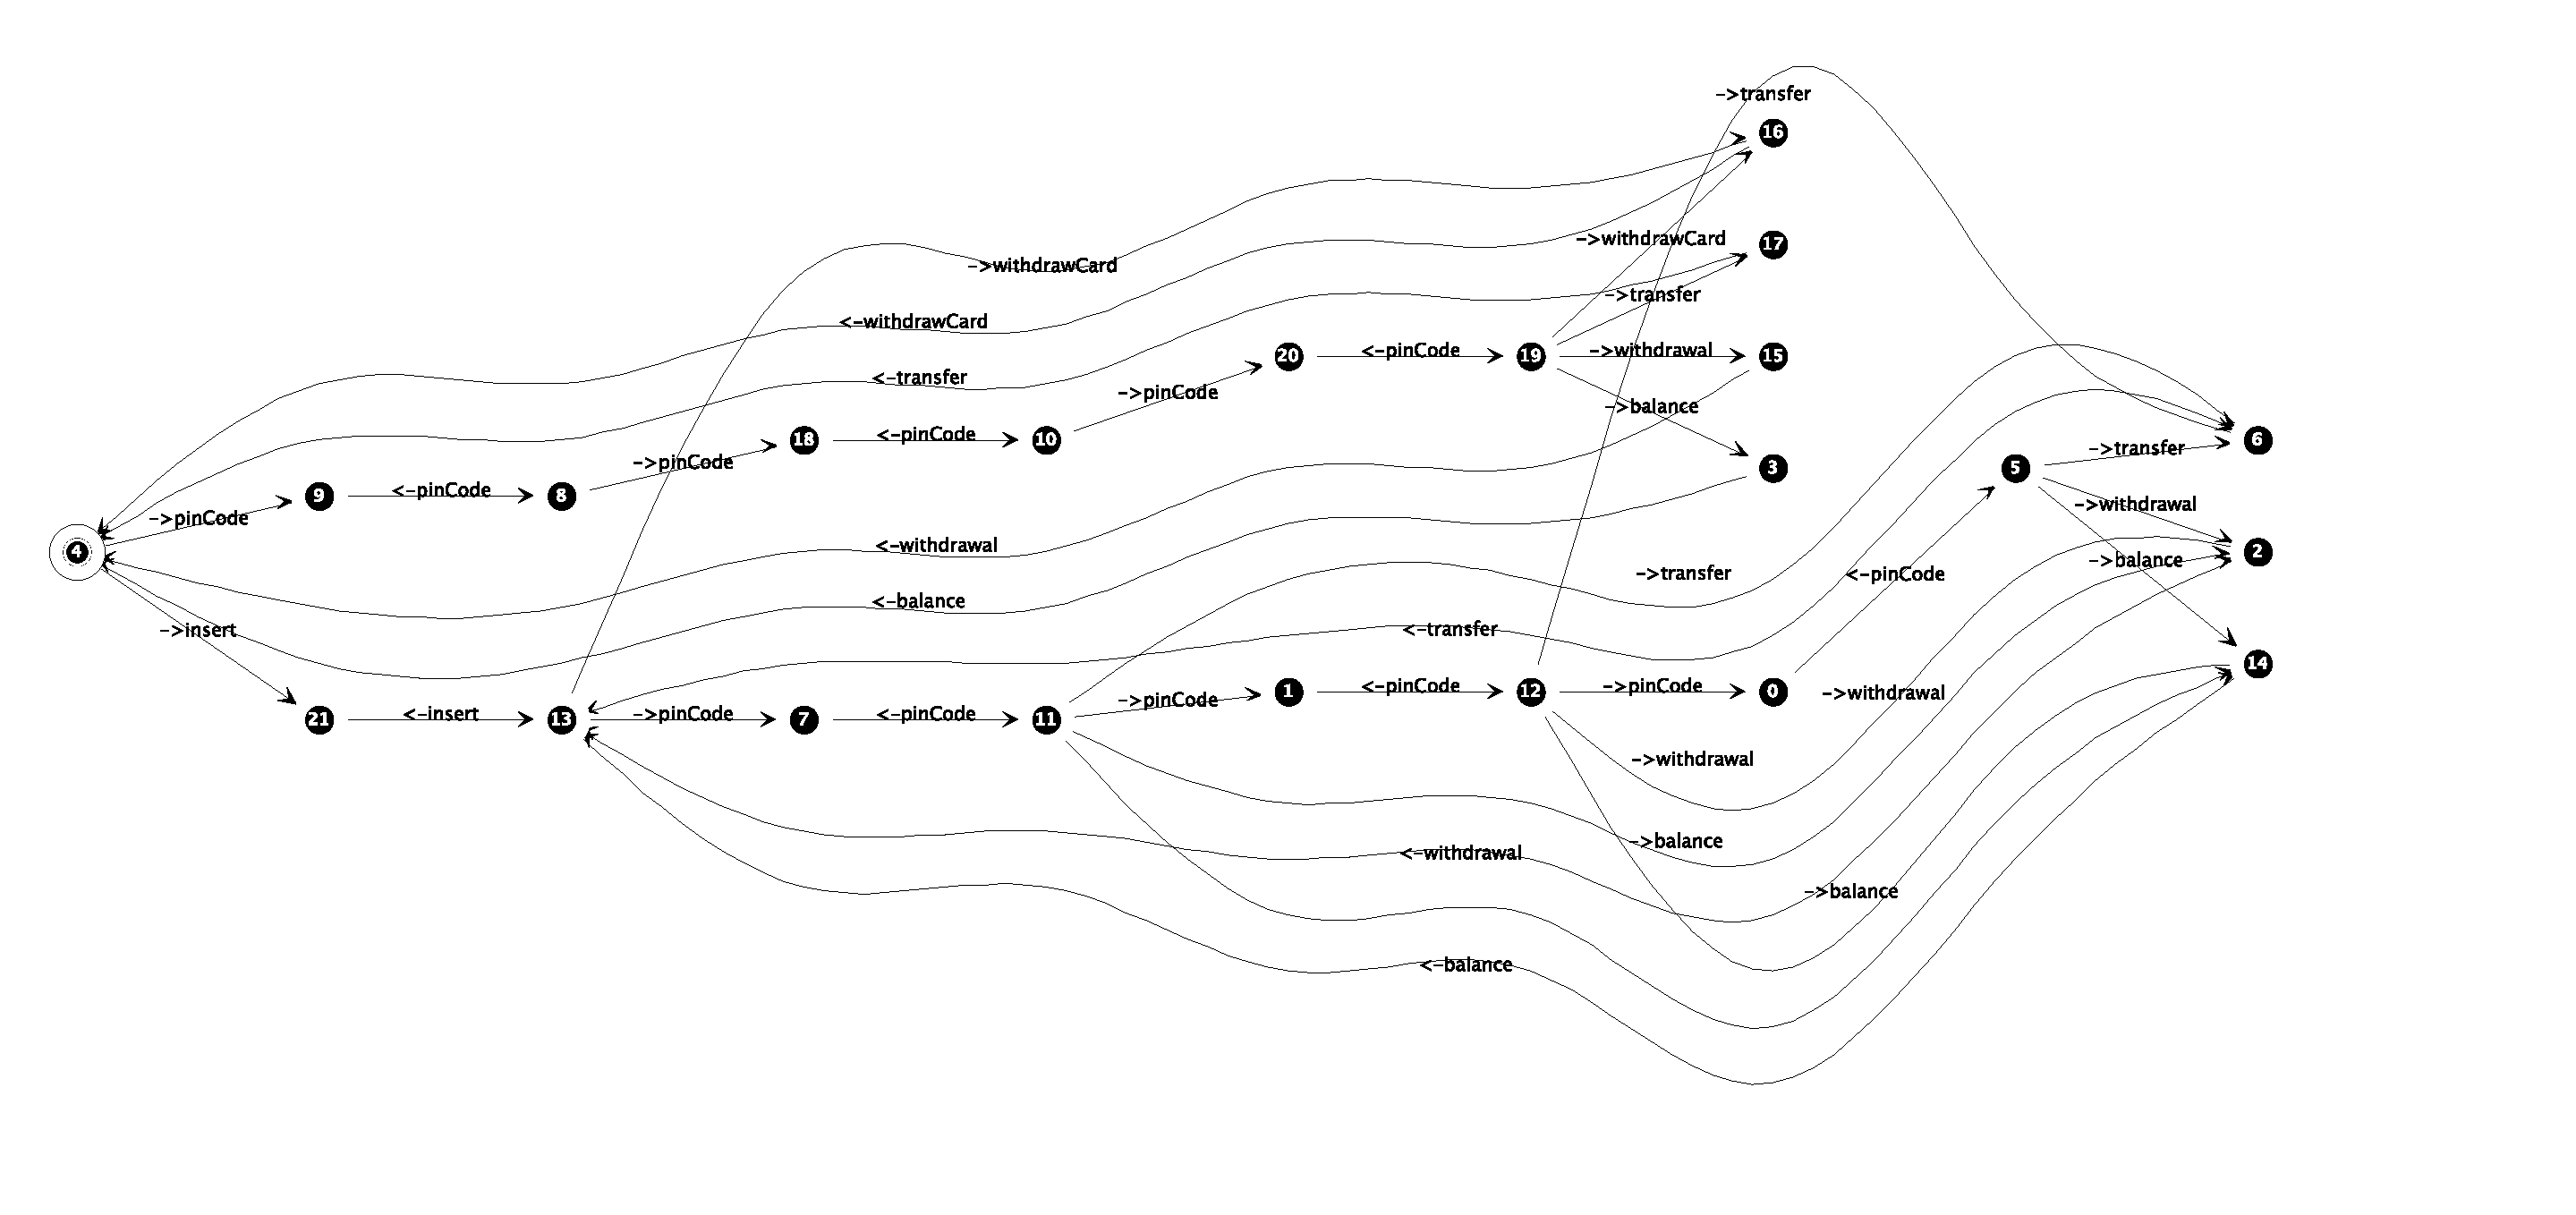
\includegraphics[width=1.2\textwidth]{figures/fig-dab-abstract-min.eps}
%%     \caption{Automate abstrait de l'interface DAB}
%%     \label{fig-auto-dab-abstract}
%% \end{figure}

%% On peut donc construire un observateur pour cette propri\'et\'e
%% d'ind\'ependance.

 
%% \subsection{Test de r\'esilience}

%% \section{Conclusion}

%% D\'efinir testeur. Les testeurs qui nous int\'eressent sont
%% sp\'ecifiques \`a la structure des composants (voir test distribu\'e)

%% D\'efinir observateur (testeur local ?)

%% D\'efinir relations de conformit\'e (cf. relation de sous-typage
%% comportemental)

%% D\'efinir testeur pour la conformit\'e (test tous les ports +
%% comportement du composant)

%% D\'efinir testeur pour l'ind\'ependance des facettes
%% (cf. composition, propri\'et\'e 2 des facettes) = test facettes 1
%% par 1 

%% D\'efinir testeur pour la r\'esilience = test 1 facette correcte et
%% les autres incorrectes

%% Probl\`eme de la compl\'etude des tests ? exhaustivit\'e wrt
%% relation de conformit\'e ?


%% %%          r\'esilience n. f.
        
%% %% D\'efinition (physique) :
%% %% Rapport de l'\'energie restitu\'ee \`a l'\'energie fournie,
%% %% apr\`es un retour rapide ou instantan\'e et complet ou presque \`a
%% %% la forme initiale d'un \'echantillon d\'eform\'e. 

        
%% %% D\'efinition (m\'edecine) :
%% %% R\'esistance d'un mat\'eriau aux chocs r\'ep\'et\'es. S'exprimant
%% %% en Kg par cm$^2$, la r\'esilience est le rapport de l'\'energie
%% %% cin\'etique absorb\'ee n\'ecessaire \`a provoquer la rupture d'un
%% %% 6mat\'eriau, \`a la surface de la section bris\'ee. 

        
%% %% D\'efinition (psychologie) :
%% %% Aptitude \`a faire face avec succ\`es \`a une situation
%% %% repr\'esentant un stress intense en raison de sa nocivit\'e ou du
%% %% risque qu'elle repr\'esente, ainsi qu'\`a se ressaisir, \`a
%% %% s'adapter et \`a r\'eussir \`a vivre et \`a se d\'evelopper
%% %% positivement en d\'epit de ces circonstances d\'efavorables. 

%% %% R\'ESILIENCE, subst. f\'em.
%% %% A. M\'ECAN., PHYS. R\'esistance d'un mat\'eriau au
%% %% choc. Coefficient de r\'esilience. Il ne serait pas normal d'utiliser
%% %% en carrosserie, en aviation, ou dans des pi\`eces de machines, des
%% %% bois qui n'auraient pas une r\'esilience suffisante (CAMPREDON, Bois,
%% %% 1948, p. 459). 
%% %% B. ZOOL. ,,Capacit\'e de reproduction d'une esp\`ece animale
%% %% inemploy\'ee en raison d'une ambiance hostile, mais susceptible d'une
%% %% expansion soudaine si cette ambiance s'am\'eliore. \og (Husson
%% %% 1970). Les Cyprinid\'es ont parmi les Poissons une forte
%% %% r\'esilience en raison du grand nombre d'\oe ufs qu'ils pondent
%% %% (Husson 1970) \fg. 
%% %% C. Au fig., rare. Force morale; qualit\'e de quelqu'un qui ne se
%% %% d\'ecourage pas, ne se laisse pas abattre. \og Dans ce deuil, une fois
%% %% encore, elle \'etonna ses amis par son imm\'ediate r\'esilience
%% %% (MAUROIS, L\'elia, 1952, p. 469 ds QUEM. DDL t. 22)\fg . 
%% %% Prononc.: []. \'Etymol. et Hist. 1906 r\'es\'elience (La Vie au
%% %% grand air, 19 janv., p. 53b ds QUEM. DDL t. 17); 1911 r\'esilience
%% %% (Lar. mens., janv., p. 20). Empr. \`a l'angl. resilience, att. dans
%% %% ce sens d\`es 1824 (NED), sp\'ecialisation de resilience \og fait
%% %% de rebondir\fg (1626, BACON, ibid.), d\'er. de resilient,
%% %% propr. \og rejaillissant, rebondissant \fg (resilient*). REY-GAGNON
%% %% Anglic. 1981. Bbg. DUB. D\'er. 1962, p. 65. 

%% \section{Exp\'erimentation}

%%% Local Variables: 
%%% mode: latex
%%% TeX-master: "these"
%%% TeX-master: "these"
%%% TeX-master: "these"
%%% TeX-master: "these"
%%% TeX-master: "these"
%%% End: 
 